\pdfoutput=1

%\documentclass[preprint,10pt]{elsarticle}
%\documentclass[10pt]{article}
%\documentclass[review]{siamart0216}
\documentclass{siamart0216}

\usepackage{fullpage}
\usepackage{hyperref}
%\let\proof\relax
%\let\endproof\relax
\usepackage{amsmath,amssymb,amsfonts,mathrsfs}%,amsthm}
\usepackage[titletoc,toc,title]{appendix}

%\usepackage{lineno}
\usepackage{array} 
\usepackage[utf8]{inputenc}
\usepackage{listings}
\usepackage{mathtools}
\usepackage{pdfpages}
\usepackage[textsize=footnotesize,color=green]{todonotes}
\usepackage{bm}
%\usepackage{tikz}
\usepackage[normalem]{ulem}
\usepackage{hhline}

%% ====================================== alg package
\usepackage{algorithm}
\usepackage[noend]{algpseudocode}
\usepackage{algorithmicx}
\algblock{ParFor}{EndParFor}
% customising the new block
\algnewcommand\algorithmicparfor{\textbf{parfor}}
\algnewcommand\algorithmicpardo{\textbf{do}}
\algnewcommand\algorithmicendparfor{\textbf{end\ parfor}}
\algrenewtext{ParFor}[1]{\algorithmicparfor\ #1\ \algorithmicpardo}
\algrenewtext{EndParFor}{\algorithmicendparfor}
%% ====================================== end alg package

\usepackage{graphicx}
\usepackage{subfig}
\usepackage{color}

%% ====================================== graphics

\usepackage{pgfplots}
\usepackage{pgfplotstable}
\definecolor{markercolor}{RGB}{124.9, 255, 160.65}
\pgfplotsset{width=10cm,compat=1.9}
\pgfplotsset{
tick label style={font=\small},
label style={font=\small},
legend style={font=\small}
}

\usetikzlibrary{calc}

\usetikzlibrary{calc}

%%% START MACRO FOR ANNOTATION OF TRIANGLE WITH SLOPE %%%.
\newcommand{\logLogSlopeTriangle}[5]
{
    % #1. Relative offset in x direction.
    % #2. Width in x direction, so xA-xB.
    % #3. Relative offset in y direction.
    % #4. Slope d(y)/d(log10(x)).
    % #5. Plot options.

    \pgfplotsextra
    {
        \pgfkeysgetvalue{/pgfplots/xmin}{\xmin}
        \pgfkeysgetvalue{/pgfplots/xmax}{\xmax}
        \pgfkeysgetvalue{/pgfplots/ymin}{\ymin}
        \pgfkeysgetvalue{/pgfplots/ymax}{\ymax}

        % Calculate auxilliary quantities, in relative sense.
        \pgfmathsetmacro{\xArel}{#1}
        \pgfmathsetmacro{\yArel}{#3}
        \pgfmathsetmacro{\xBrel}{#1-#2}
        \pgfmathsetmacro{\yBrel}{\yArel}
        \pgfmathsetmacro{\xCrel}{\xArel}

        \pgfmathsetmacro{\lnxB}{\xmin*(1-(#1-#2))+\xmax*(#1-#2)} % in [xmin,xmax].
        \pgfmathsetmacro{\lnxA}{\xmin*(1-#1)+\xmax*#1} % in [xmin,xmax].
        \pgfmathsetmacro{\lnyA}{\ymin*(1-#3)+\ymax*#3} % in [ymin,ymax].
        \pgfmathsetmacro{\lnyC}{\lnyA+#4*(\lnxA-\lnxB)}
        \pgfmathsetmacro{\yCrel}{\lnyC-\ymin)/(\ymax-\ymin)} % THE IMPROVED EXPRESSION WITHOUT 'DIMENSION TOO LARGE' ERROR.

        % Define coordinates for \draw. MIND THE 'rel axis cs' as opposed to the 'axis cs'.
        \coordinate (A) at (rel axis cs:\xArel,\yArel);
        \coordinate (B) at (rel axis cs:\xBrel,\yBrel);
        \coordinate (C) at (rel axis cs:\xCrel,\yCrel);

        % Draw slope triangle.
        \draw[#5]   (A)-- node[pos=0.5,anchor=north] {1}
                    (B)-- 
                    (C)-- node[pos=0.5,anchor=west] {#4}
                    cycle;
    }
}
%%% END MACRO FOR ANNOTATION OF TRIANGLE WITH SLOPE %%%.

\newcommand{\logLogSlopeTriangleNeg}[5]
{
    % #1. Relative offset in x direction.
    % #2. Width in x direction, so xA-xB.
    % #3. Relative offset in y direction.
    % #4. Slope d(y)/d(log10(x)).
    % #5. Plot options.

    \pgfplotsextra
    {
        \pgfkeysgetvalue{/pgfplots/xmin}{\xmin}
        \pgfkeysgetvalue{/pgfplots/xmax}{\xmax}
        \pgfkeysgetvalue{/pgfplots/ymin}{\ymin}
        \pgfkeysgetvalue{/pgfplots/ymax}{\ymax}

        % Calculate auxilliary quantities, in relative sense.
        \pgfmathsetmacro{\xArel}{#1}
        \pgfmathsetmacro{\yArel}{#3}
        \pgfmathsetmacro{\xBrel}{#1-#2}
        \pgfmathsetmacro{\yBrel}{\yArel}
        \pgfmathsetmacro{\xCrel}{\xArel}

        \pgfmathsetmacro{\lnxB}{\xmin*(1-(#1-#2))+\xmax*(#1-#2)} % in [xmin,xmax].
        \pgfmathsetmacro{\lnxA}{\xmin*(1-#1)+\xmax*#1} % in [xmin,xmax].
        \pgfmathsetmacro{\lnyA}{\ymin*(1-#3)+\ymax*#3} % in [ymin,ymax].
        \pgfmathsetmacro{\lnyC}{\lnyA+#4*(\lnxA-\lnxB)}
        \pgfmathsetmacro{\yCrel}{\lnyC-\ymin)/(\ymax-\ymin)} % THE IMPROVED EXPRESSION WITHOUT 'DIMENSION TOO LARGE' ERROR.

        % Define coordinates for \draw. MIND THE 'rel axis cs' as opposed to the 'axis cs'.
        \coordinate (A) at (rel axis cs:\xArel,\yArel);
        \coordinate (B) at (rel axis cs:\xBrel,\yBrel);
        \coordinate (C) at (rel axis cs:\xCrel,\yCrel);

        % Draw slope triangle.
        \draw[#5]   (A)-- node[pos=.5,anchor=south] {1}
                    (B)-- 
                    (C)-- node[pos=0.5,anchor=west] {#4}
                    cycle;
    }
}
%%% END MACRO FOR ANNOTATION OF TRIANGLE WITH SLOPE %%%.

%%% START MACRO FOR ANNOTATION OF TRIANGLE WITH SLOPE %%%.
\newcommand{\logLogSlopeTriangleFlipNeg}[5]
{
    % #1. Relative offset in x direction.
    % #2. Width in x direction, so xA-xB.
    % #3. Relative offset in y direction.
    % #4. Slope d(y)/d(log10(x)).
    % #5. Plot options.

    \pgfplotsextra
    {
        \pgfkeysgetvalue{/pgfplots/xmin}{\xmin}
        \pgfkeysgetvalue{/pgfplots/xmax}{\xmax}
        \pgfkeysgetvalue{/pgfplots/ymin}{\ymin}
        \pgfkeysgetvalue{/pgfplots/ymax}{\ymax}

        % Calculate auxilliary quantities, in relative sense.
        %\pgfmathsetmacro{\xArel}{#1}
        %\pgfmathsetmacro{\yArel}{#3}
        \pgfmathsetmacro{\xBrel}{#1-#2}
        \pgfmathsetmacro{\yBrel}{#3}
        \pgfmathsetmacro{\xCrel}{#1}

        \pgfmathsetmacro{\lnxB}{\xmin*(1-(#1-#2))+\xmax*(#1-#2)} % in [xmin,xmax].
        \pgfmathsetmacro{\lnxA}{\xmin*(1-#1)+\xmax*#1} % in [xmin,xmax].
        \pgfmathsetmacro{\lnyA}{\ymin*(1-#3)+\ymax*#3} % in [ymin,ymax].
        \pgfmathsetmacro{\lnyC}{\lnyA+#4*(\lnxA-\lnxB)}
        \pgfmathsetmacro{\yCrel}{\lnyC-\ymin)/(\ymax-\ymin)} % THE IMPROVED EXPRESSION WITHOUT 'DIMENSION TOO LARGE' ERROR.

	\pgfmathsetmacro{\xArel}{\xBrel}
        \pgfmathsetmacro{\yArel}{\yCrel}

        % Define coordinates for \draw. MIND THE 'rel axis cs' as opposed to the 'axis cs'.
        \coordinate (A) at (rel axis cs:\xArel,\yArel);
        \coordinate (B) at (rel axis cs:\xBrel,\yBrel);
        \coordinate (C) at (rel axis cs:\xCrel,\yCrel);

        % Draw slope triangle.
        \draw[#5]   (A)-- node[pos=0.5,anchor=east] {#4}
                    (B)-- 
                    (C)-- node[pos=0.5,anchor=north] {1}
                    cycle;
    }
}
%%% END MACRO FOR ANNOTATION OF TRIANGLE WITH SLOPE %%%.


%%% START MACRO FOR ANNOTATION OF TRIANGLE WITH SLOPE %%%.
\newcommand{\logLogSlopeTriangleFlip}[5]
{
    % #1. Relative offset in x direction.
    % #2. Width in x direction, so xA-xB.
    % #3. Relative offset in y direction.
    % #4. Slope d(y)/d(log10(x)).
    % #5. Plot options.

    \pgfplotsextra
    {
        \pgfkeysgetvalue{/pgfplots/xmin}{\xmin}
        \pgfkeysgetvalue{/pgfplots/xmax}{\xmax}
        \pgfkeysgetvalue{/pgfplots/ymin}{\ymin}
        \pgfkeysgetvalue{/pgfplots/ymax}{\ymax}

        % Calculate auxilliary quantities, in relative sense.
        %\pgfmathsetmacro{\xArel}{#1}
        %\pgfmathsetmacro{\yArel}{#3}
        \pgfmathsetmacro{\xBrel}{#1-#2}
        \pgfmathsetmacro{\yBrel}{#3}
        \pgfmathsetmacro{\xCrel}{#1}

        \pgfmathsetmacro{\lnxB}{\xmin*(1-(#1-#2))+\xmax*(#1-#2)} % in [xmin,xmax].
        \pgfmathsetmacro{\lnxA}{\xmin*(1-#1)+\xmax*#1} % in [xmin,xmax].
        \pgfmathsetmacro{\lnyA}{\ymin*(1-#3)+\ymax*#3} % in [ymin,ymax].
        \pgfmathsetmacro{\lnyC}{\lnyA+#4*(\lnxA-\lnxB)}
        \pgfmathsetmacro{\yCrel}{\lnyC-\ymin)/(\ymax-\ymin)} % THE IMPROVED EXPRESSION WITHOUT 'DIMENSION TOO LARGE' ERROR.

	\pgfmathsetmacro{\xArel}{\xBrel}
        \pgfmathsetmacro{\yArel}{\yCrel}

        % Define coordinates for \draw. MIND THE 'rel axis cs' as opposed to the 'axis cs'.
        \coordinate (A) at (rel axis cs:\xArel,\yArel);
        \coordinate (B) at (rel axis cs:\xBrel,\yBrel);
        \coordinate (C) at (rel axis cs:\xCrel,\yCrel);

        % Draw slope triangle.
        \draw[#5]   (A)-- node[pos=0.5,anchor=east] {#4}
                    (B)-- 
                    (C)-- node[pos=0.5,anchor=south] {1}
                    cycle;
    }
}
%%% END MACRO FOR ANNOTATION OF TRIANGLE WITH SLOPE %%%.



\usepackage{stmaryrd}


\renewcommand{\topfraction}{0.85}
\renewcommand{\textfraction}{0.1}
\renewcommand{\floatpagefraction}{0.75}

\newcommand{\vect}[1]{\ensuremath\boldsymbol{#1}}
\newcommand{\tensor}[1]{\underline{\bm{#1}}}
\newcommand{\del}{\triangle}
\newcommand{\curl}{\grad \times}
\renewcommand{\div}{\grad \cdot}
\newcommand{\td}[2]{\frac{{\rm d}#1}{{\rm d}{\rm #2}}}
\newcommand{\pd}[2]{\frac{\partial#1}{\partial#2}}
\newcommand{\pdd}[2]{\frac{\partial^2#1}{\partial#2^2}}

\newcommand{\bs}[1]{\boldsymbol{#1}}

\newcommand{\equaldef}{\stackrel{\mathrm{def}}{=}}



\newcommand{\mi}{\mathrm{i}} %% roman "i"
\newcommand{\mb}[1]{\mathbf{#1}}
\newcommand{\mbb}[1]{\mathbb{#1}}
\newcommand{\mc}[1]{\mathcal{#1}}
\newcommand{\nor}[1]{\left\| #1 \right\|}
\newcommand{\LRp}[1]{\left( #1 \right)}
\newcommand{\LRs}[1]{\left[ #1 \right]}
\newcommand{\LRa}[1]{\left\langle #1 \right\rangle}
\newcommand{\LRb}[1]{\left| #1 \right|}
\newcommand{\LRc}[1]{\left\{ #1 \right\}}
\newcommand{\LRceil}[1]{\left\lceil #1 \right\rceil}
\newcommand{\LRl}[1]{\left. #1 \right|}

%\newcommand{\cond}[1]{\kappa\LRp{#1}}
\newcommand{\cond}[2]{\nor{#1}_{#2}\nor{{#1}^{-1}}_{#2}}


\newcommand{\Grad} {\ensuremath{\nabla}}
\newcommand{\Div} {\ensuremath{\nabla\cdot}}
\newcommand{\jump}[1] {\ensuremath{\llbracket#1\rrbracket}}
\newcommand{\avg}[1] {\ensuremath{\LRc{\!\{#1\}\!}}}

\renewcommand{\Oh}{{\Omega_h}}
\renewcommand{\L}{L^2\LRp{\Omega}}
%\newcommand{\Lk}{\Lk}
%\newcommand{\Ldk}{L^2\LRp{\partial D^k}}
\newcommand{\Lk}{D^k}
\newcommand{\Ldk}{\partial D^k}
\newcommand{\Dhat}{\widehat{D}}
\newcommand{\Lhat}{L^2\LRp{\Dhat}}

%\newtheorem{theorem}{Theorem}[section]
%\newtheorem{lemma}[theorem]{Lemma}
%\newtheorem{proposition}[theorem]{Proposition}
%\newtheorem{corollary}[theorem]{Corollary}

%\newenvironment{definition}[1][Definition]{\begin{trivlist}
%\item[\hskip \labelsep {\bfseries #1}]}{\end{trivlist}}
%\newenvironment{example}[1][Example]{\begin{trivlist}
%\item[\hskip \labelsep {\bfseries #1}]}{\end{trivlist}}

\newcommand{\eval}[2][\right]{\relax
  \ifx#1\right\relax \left.\fi#2#1\rvert}

\def\etal{{\it et al.~}}


\newcommand{\note}[1]{{\color{blue}{#1}}}
\newcommand{\remark}[1]{\textbf{\color{red}#1}}


\newcommand{\LinfDk}{L^{\infty}\LRp{D^k}}

\newcommand{\diag}[1]{{\rm diag}\LRp{#1}}

\newcommand{\half}{1/2}

\newcolumntype{C}[1]{>{\centering\let\newline\\\arraybackslash\hspace{0pt}}m{#1}}

%% d in integrand
\newcommand*\diff[1]{\mathop{}\!{\mathrm{d}#1}}

\makeatletter
\renewcommand\d[1]{\mspace{6mu}\mathrm{d}#1\@ifnextchar\d{\mspace{-3mu}}{}}
\makeatother

\date{}
\author{Jesse Chan}
\title{Weight-adjusted discontinuous Galerkin methods: matrix-valued weights and linear elastic wave propagation}

\begin{document}

\maketitle

\begin{abstract}
Weight-adjusted inner products \cite{chan2016weight1,chan2016weight2} replace weighted $L^2$ inner products with easily invertible weight-adjusted approximations.  When paired with discontinuous Galerkin (DG) methods, the result is a low storage, energy stable, and (for sufficiently regular weights) high order accurate method for wave propagation in the presence of general heterogeneous media and curvilinear meshes.  In this work, we extend weight-adjusted DG (WADG) methods to weighted inner products with matrix-valued weights, focusing on the linear elastic wave equation as an application.  We present a new DG formulation based on the discretization of the symmetric form of the linear elasticity wave equation, with upwind-like dissipation incorporated through simple penalty terms in the numerical fluxes.  This results in provably stable formulations for arbitrary anisotropic stiffness tensors and curvilinear meshes.  A convergence analysis is given, and numerical results confirm the stability and high order accuracy of WADG for several problems in elastic wave propagation.  
\end{abstract}

%\tableofcontents


\section{Introduction}

There exist many high order energy stable discontinuous Galerkin formulations for the elastic wave equations in first order form.  Wilcox et al.\ introduced a discontinuous Galerkin spectral element method on hexahedral meshes 

SEM \cite{komatitsch2010high}

DG-SEM \cite{wilcox2010high} 

High order DG \cite{kaser2006arbitrary, dumbser2006arbitrary, de2007arbitrary, ye2016discontinuous}

Interior penalty formulations.  Analysis: Riviere et al.\ \cite{riviere2003discontinuous,riviere2007discontinuous} and Delcourte et al.\ \cite{delcourte2009high,delcourte2015analysis}

GPU-accelerated DG methods \cite{klockner2009nodal,godel2010gpu,godel2010scalability}.  Also elastic wave propagation and seismic wave applications \cite{modave2015nodal, modave2016gpu}

High order approximations of material data \cite{castro2010seismic, mercerat2015nodal}, but not low storage or not energy stable.  

Extending mass lumping without dispersive effects \cite{christon1999influence,guermond2013correction}.  Reduces to exact mass matrix inversion for constant weights.  


A simpler extension of WADG \cite{chan2016weight1,chan2016weight2} to elasticity and weight-adjusted inner products for vector-valued functions.  


Outline: present elasticity and an energy stable DG method, motivate need for alternative to inverting large dense coupled mass matrix, introduce weight-adjusted inner products.  

\section{Symmetric form of the elastic wave equation }

We begin with the linear elastic wave equation under small deformations in a domain $\Omega$.  These equations can be written a first order velocity-stress system for velocity $\bm{v}$ and symmetric stress tensor $\bm{S}$ 
\begin{align*}
\rho \pd{\bm{v}}{t} &= \Div{\bm{S}} + \bm{f}\\
\pd{\bm{S}}{t} &= \frac{1}{2} \bar{\bm{C}}\LRp{\Grad\bm{v} + \Grad\bm{v}^T},
\end{align*}
where $\bm{f}$ is the body force per unit volume, $\rho$ is density, and $\bar{\bm{C}}$ is the symmetric constitutive stiffness tensor relating stress and strain.  These equations can also be rewritten as a symmetric hyperbolic system of PDEs \cite{hughes1978classical}  
\begin{align}
\rho \pd{\bm{v}}{t} &= \sum_{i=1}^d \bm{A}_i^T \pd{\bm{\sigma}}{\bm{x}_i}\nonumber + \bm{f}\\
\bm{C}^{-1} \pd{\bm{\sigma}}{t} &= \sum_{i=1}^d \bm{A}_i \pd{\bm{v}}{\bm{x}_i}.
\label{eq:symelas}
\end{align}
where $\bm{C}$ is the symmetric matrix form of the constitutive tensor $\bar{\bm{C}}$ and $\sigma$ is a vector of length $N_d = \frac{d(d+1)}{2}$, the number of unique entries of the stress tensor $\bm{S}$.  We note that the matrices $\bm{A}_i$ are constant, while $\rho$ and $\bm{C}$ can vary spatially.  Furthermore, we will assume that $\rho$ and $\bm{C}$ are positive-definite and bounded such that 
\begin{align*}
\rho_{\min} &\leq \rho(\bm{x}) \leq \rho_{\max} \\
0 < c_{\min} \leq \bm{x}^T\bm{C}\bm{x} &\leq c_{\max} < \infty, \qquad \bm{x} \in \mathbb{R}^{N_d},
\end{align*}
which also implies that $\bm{C}^{-1}$ is positive-definite and bounded.

In two dimensions, $\bm{v} = (\bm{v}_1, \bm{v}_2)^T$ and $\bm{\sigma}= (\sigma_{xx},\sigma_{yy},\sigma_{xy})^T$ 
\[
\bm{S} = \LRp{\begin{array}{cc}
\sigma_{xx} & \sigma_{xy}\\
\sigma_{xy} & \sigma_{yy}
\end{array}}.
\]
The matrices $\bm{A}_i$ are given as
\[
\bm{A}_1 = \left(\begin{array}{cc}
1 & 0\\
0 & 0\\
0 & 1
\end{array}\right), \qquad 
\bm{A}_2 = \left(\begin{array}{cc}
0 & 0\\
0 & 1\\
1 & 0
\end{array}\right).
\]

In three dimensions, the velocity is $\bm{v} = (\bm{v}_1,\bm{v}_2,\bm{v}_3)^T$, while $\bm{\sigma}= (\sigma_{xx},\sigma_{yy},\sigma_{zz},\sigma_{yz},\sigma_{xy},\sigma_{xz})^T$ denotes the unique entries of the stress tensor $\bm{S}$
\[
\bm{S} = \LRp{\begin{array}{ccc}
\sigma_{xx} & \sigma_{xy} & \sigma_{xz}\\
\sigma_{xy} & \sigma_{yy}& \sigma_{yz}\\
\sigma_{xz} & \sigma_{yz}& \sigma_{zz}
\end{array}}.
\]
The matrices $\bm{A}_i$ are then
\[
\bm{A}_1 = \left(\begin{array}{ccc}
1 & 0 & 0\\
0 & 0& 0\\
0 & 0& 0\\
0 & 0& 0\\
0 & 0 & 1\\
0 & 1 & 0
\end{array}\right), \qquad 
\bm{A}_2 = \left(\begin{array}{ccc}
0 & 0 & 0\\
0 & 1 & 0\\
0 & 0 & 0\\
0 & 0 & 1\\
0 & 0 & 0\\
1 & 0 & 0
\end{array}\right), \qquad
\bm{A}_3 = \left(\begin{array}{ccc}
0 & 0 & 0\\
0 & 0 & 0\\
0 & 0 & 1\\
0 & 1 & 0\\
1 & 0 & 0\\
0 & 0 & 0
\end{array}\right)
\]

In general anisotropic media, $\bm{C}$ is symmetric and positive-definite.  For two-dimensional isotropic media, $\bm{C}$ is given as
\[
\bm{C}= \LRp{
\begin{array}{ccc}
2\mu+\lambda  &  \lambda  &     0\\
\lambda &       2\mu+\lambda &      0\\
          0 &      0           &     {\mu}
\end{array}}, 
\]
where $\lambda,\mu$ are Lame parameters.  For three-dimensional isotropic media, $\bm{C}$ is given instead by
\[
\bm{C}= \LRp{
\begin{array}{cccccc}
2\mu+\lambda  &  \lambda  &     \lambda  & & & \\
\lambda &   2\mu+\lambda & \lambda   & & & \\
\lambda & \lambda &   2\mu+\lambda &    & &\\
 &   &    & {\mu} & &\\
&  &   &    & {\mu} &\\
& &  &   &    & {\mu} \\
\end{array}}.  
\]
We will consider both spatially varying isotropic and anisotropic media in this work.  

\section{An energy stable discontinuous Galerkin formulation for elastic wave propagation}

The advantage of the symmetric first order formulation of the elastic wave equations (\ref{eq:symelas}) is that it is straightforward to derive an energy stable discontinuous Galerkin formulation.  We assume that the domain $\Omega$ is Lipschitz and exactly triangulated by a mesh $\Omega_h$, which consists of elements $D^k$.  We further assume that each element $D^k$ is the image of a reference element $\widehat{D}$ under the local elemental mapping 
\[
\bm{x}^k = \bm{\Phi}^k \widehat{\bm{x}},
\]
where $\bm{x}^k = \LRc{x^k,y^k,z^k}$ denote physical coordinates on $D^k$ and $\widehat{\bm{x}} = \LRc{\widehat{x},\widehat{y},\widehat{z}}$ denote coordinates on the reference element.  We denote the determinant of the Jacobian of $\bm{\Phi}^k$ as $J$, and refer to it as the Jacobian for the remainder of this work.  

We will approximate components over each element $D^k$ from an approximation space $V_h\LRp{D^k}$, which we define as the composition of the mapping $\bm{\Phi}^k$ and a reference approximation space $V_h\LRp{\widehat{D}}$
\[
V_h\LRp{D^k} = \bm{\Phi}^k \circ V_h\LRp{\widehat{D}}.
\]
For the remainder of this work, we will take $V_h\LRp{\widehat{D}} = P^N\LRp{\widehat{D}}$, where $P^N\LRp{\widehat{D}}$ is the polynomial space of total degree $N$ on the reference simplex.  In two dimensions, 
\[
P^N\LRp{\widehat{D}} = \LRc{ \widehat{x}^i \widehat{y}^j, \quad 0 \leq i + j \leq N},
\] 
and in three dimensions, 
\[
P^N\LRp{\widehat{D}} = \LRc{ \widehat{x}^i \widehat{y}^j \widehat{z}^k, \quad 0 \leq i + j +k \leq N}.  
\]

We denote the $L^2$ inner product and norm over $D^k$ by $\LRp{\cdot,\cdot}_{\Lk}$, such that
\[
\LRp{\bm{f},\bm{g}}_{\Lk} = \int_{D^k} \bm{f}\cdot\bm{g} \diff x = \int_{\widehat{D}} \bm{f}\cdot\bm{g} J, \qquad \nor{\bm{f}}_{\Lk}^2 = \LRp{\bm{f},\bm{f}}_{\Lk},
\]
where $\bm{f},\bm{g}$ are vector-valued functions.  Global $L^2$ inner products and norms are using local $L^2$ inner products and norms
\[
\LRp{\bm{f},\bm{g}}_{\Oh} = \sum_{D^k\in \Oh} \int_{D^k} \LRp{\bm{f},\bm{g}}_{\Lk}, \qquad \nor{\bm{f}}_{\Oh}^2 = \sum_{D^k\in \Oh} \nor{\bm{f}}^2_{\Lk}.
\]

Let $f$ be a face of an element $D^{k}$ with neighboring element $D^{k,+}$ and unit outward normal $\bm{n}$.  We define $u^-$ and $u^+$ denote interior and exterior values of a discontinuous function $u$ such that
\[
{u}^- = \LRl{u}_{f \cap D^k}, \qquad {u}^+ = \LRl{u}_{f \cap  \partial D^{k,+}}.  
\]
The jump and average of a scalar function $u\in V_h\LRp{\Omega_h}$ over $f$ are then defined as
\[
\jump{u} = u^+ - u^-, \qquad \avg{u} = \frac{u^+ + u^-}{2}.
\]
Jumps and averages of a vector-valued functions $\bm{u}\in \mathbb{R}^m$ and $\bm{S}\in \mathbb{R}^{m\times n}$ are then defined component-wise 
\[
\LRp{\jump{\bm{u}}}_i = \jump{\bm{u}_i}, \qquad 1\leq i \leq m, \qquad \LRp{\jump{\bm{S}}}_{ij} = \jump{\bm{S}_i}, \qquad 1\leq i \leq m, \quad 1\leq j \leq n.
\]

We can now specify a DG formulation for the linear elastic wave equation (\ref{eq:symelas}).  Symmetric hyperbolic systems readily admit a DG formulation based on penalty fluxes, as detailed in \cite{chan2016short}.  For the linear elastic wave equation in symmetric first order form, this formulation is given as
\begin{align}
\sum_{D^k\in \Oh} \LRp{\rho \pd{\bm{v}}{t},\bm{w}}_{\Lk} &= 
\sum_{D^k\in \Oh} \LRp{\LRp{ \sum_{i=1}^d \bm{A}_i^T\pd{\bm{\sigma}}{\bm{x}_i} + \bm{f},\bm{w}}_{\Lk}  + \LRa{\frac{1}{2}\bm{A}_n^T\jump{\bm{\sigma}} + \frac{\tau_v}{2}\bm{A}_n^T\bm{A}_n\jump{\bm{v}},\bm{w}}_{\Ldk}} \nonumber\\
\sum_{D^k\in \Oh}\LRp{\bm{C}^{-1} \pd{\bm{\sigma}}{t},\bm{q}}_{\Lk} &=
\sum_{D^k\in \Oh}\LRp{\LRp{\sum_{i=1}^d \bm{A}_i \pd{\bm{v}}{\bm{x}_i},\bm{q}}_{\Lk} + \LRa{\frac{1}{2}\bm{A}_n\jump{\bm{v}} + \frac{\tau_{\sigma}}{2}\bm{A}_n\bm{A}_n^T\jump{\bm{\sigma}},\bm{q}}_{\Ldk}},
\label{eq:dgform}
\end{align}
for all $\bm{w},\bm{q}\in V_h\LRp{\Omega_h}$.  Here, $\tau_v,\tau_\sigma \geq 0$ are penalty parameters and $\bm{A}_n$ is the normal matrix defined on a face $f$ as $\bm{A}_n = \sum_{i=1}^d \bm{n}_i \bm{A}_i$.  In two dimensions, $\bm{A}_n$ is 
\[
\bm{A}_n =  \LRp{\begin{array}{cc}
{n}_x & 0\\
 0 & {n}_y\\
{n}_y & {n}_x
\end{array}}.
\]
while in three dimensions, $\bm{A}_n$ is
\[
\bm{A}_n =  \LRp{\begin{array}{ccc}
{n}_x & 0 & 0\\
 0 & {n}_y & 0\\
0&  0 & {n}_z \\
0 &{n}_z & {n}_y\\
{n}_z & 0 & {n}_x\\
{n}_y & {n}_z & 0\\
\end{array}}.  
\]

\subsection{Boundary conditions}

In this work, we assume boundary conditions on velocity and traction of the form
\[
\bm{v} = \bm{v}_{\rm bc}, \qquad \bm{S}\bm{n} = \bm{t}_{\rm bc}
\]
where $\bm{v}_{\rm bc}$ and $\bm{t}_{\rm bc}$ are given values.  Traction boundary conditions where $\bm{t}_{\rm bc} = 0$ are referred to as free-surface boundary conditions.  We follow \cite{leveque2002finite,wilcox2010high} and impose boundary conditions on the DG formulation through exterior values and jumps of the solution.  Boundary conditions on the normal component of the stress can be imposed by noting that the numerical flux contains the term $\jump{\bm{A}_n^T\bm{\sigma}} = \bm{S}\bm{n}$.  

For a face which lies on a boundary, velocity boundary conditions are imposed by setting 
\begin{align*}
\jump{\bm{v}} &= 2\LRp{\bm{v}_{\rm bc} - \bm{v}^- }, \qquad \jump{\bm{A}_n^T\bm{\sigma}}=\jump{\bm{S}\bm{n}} = 0, 
\end{align*}
while traction boundary conditions are imposed by
\begin{align*}
\jump{\bm{A}_n^T\bm{\sigma}} = \jump{\bm{S}\bm{n}} = 2\LRp{\bm{t}_{\rm bc} - \bm{S}^-\bm{n} }= 2\LRp{\bm{t}_{\rm bc} - \bm{A}_n^T\bm{\sigma}^- }, \qquad \jump{\bm{v}} = 0.
\end{align*}
For problems which involve the truncation of infinite or large domains, absorbing boundary conditions are required.  For such cases, we impose simple non-reflective boundary conditions \cite{leveque2002finite} through jumps 
\begin{align*}
\jump{\bm{A}_n^T\bm{\sigma}} = \jump{\bm{S}\bm{n}} = - \bm{S}^-\bm{n} = -\bm{A}_n^T\bm{\sigma}^- , \qquad \jump{\bm{v}} = - \bm{v}^-. 
\end{align*}
We note that more accurate absorbing conditions can be imposed using, for example, perfectly matched layers \cite{berenger1994perfectly} or high order absorbing boundary conditions \cite{hagstrom2004new,modave2016high}.  

In all cases, boundary conditions are imposed by computing numerical fluxes using these modified jumps.  This imposition guarantees energy stability for all three sets of boundary conditions.


%Easiest way to impose BCs: set $U^+$ values, compute central fluxes and then compute penalty fluxes via $\bm{A}_n^T\bm{A}_n \jump{U} = \bm{A}_n \jump{F}$.  


\subsection{Energy stability}

It is straightforward to show that the formulation (\ref{eq:dgform}) is energy stable for zero velocity and traction boundary conditions, as well as non-reflective boundary conditions.  Integrating by parts the velocity equations gives
\begin{align*}
\LRp{\rho \pd{\bm{v}}{t},\bm{w}}_{\Lk} &= -\LRp{ \sum_{i=1}^d \bm{\sigma},\bm{A}_i \pd{\bm{w}}{\bm{x}_i}}_{\Lk}  + \LRa{\bm{A}_n^T\avg{\bm{\sigma}} + \frac{\tau_v}{2}\bm{A}_n^T\bm{A}_n\jump{\bm{v}},\bm{w}}_{\Ldk} \nonumber\\
\LRp{\bm{C}^{-1} \pd{\bm{\sigma}}{t},\bm{q}}_{\Lk} &= \LRp{\sum_{i=1}^d \bm{A}_i \pd{\bm{v}}{\bm{x}_i},\bm{q}}_{\Lk} + \LRa{\frac{1}{2}\bm{A}_n\jump{\bm{v}} + \frac{\tau_{\sigma}}{2}\bm{A}_n\bm{A}_n^T\jump{\bm{\sigma}},\bm{q}}_{\Ldk} 
\end{align*}
Taking $(\bm{w},\bm{q}) = (\bm{v},\bm{\sigma})$ and adding both equations together yields
\begin{align*}
\sum_{D^k\in \Oh}\frac{1}{2}\pd{}{t}&\LRp{\LRp{\rho \bm{v},\bm{v}}_{\Lk} + \LRp{\bm{C}^{-1} \bm{\sigma},\bm{\sigma}}_{\Lk}} =  \\
&\sum_{D^k\in \Omega_h}\LRa{\bm{A}_n^T\avg{\bm{\sigma}} + \frac{\tau_v}{2}\bm{A}_n^T\bm{A}_n\jump{\bm{v}},\bm{v}}_{\partial D^k}+ \LRa{\frac{1}{2}\bm{A}_n\jump{\bm{v}} + \frac{\tau_\sigma}{2}\bm{A}_n\bm{A}_n^T\jump{\bm{\sigma}},\bm{\sigma}}_{\partial D^k}  \\
&\sum_{D^k\in \Omega_h}\sum_{f\in \partial D^k}\int_{f}{\bm{A}_n^T\avg{\bm{\sigma}}\bm{v} + \frac{\tau_v}{2}\bm{A}_n^T\bm{A}_n\jump{\bm{v}}\bm{v}} + {\frac{1}{2}\bm{A}_n\jump{\bm{v}}\bm{\sigma} + \frac{\tau_\sigma}{2}\bm{A}_n\bm{A}_n^T\jump{\bm{\sigma}}\bm{\sigma}}.
\end{align*}
Let $\Gamma_h$ denote the set of unique faces in $\Oh$, and let $\Gamma_v,\Gamma_\sigma,\Gamma_{\rm abc}$ denote the parts of the boundary where velocity, traction, and non-reflective boundary conditions are imposed, respectively.  We separate surface terms into contributions from interior shared faces and from boundary faces.  On an interior shared face, we sum contributions from the two adjacent elements to yield
\begin{align*}
&\sum_{f\in \Gamma_h \setminus \partial \Omega} \int_{f}{\bm{A}_n^T\avg{\bm{\sigma}}\bm{v} + \frac{\tau_v}{2}\bm{A}_n^T\bm{A}_n\jump{\bm{v}}\bm{v}} + {\frac{1}{2}\bm{A}_n\jump{\bm{v}}\bm{\sigma} + \frac{\tau_\sigma}{2}\bm{A}_n\bm{A}_n^T\jump{\bm{\sigma}}\bm{\sigma}}\\
&\leq - \sum_{f \in\Gamma_h \setminus \partial \Omega} \int_{f} \frac{\tau_v}{2}\LRb{\bm{A}_n\jump{\bm{v}}}^2 + \frac{\tau_\sigma}{2}\LRb{\bm{A}_n^T\jump{\bm{\sigma}}}^2.  
%\label{thm:stability}
\end{align*}
For faces which lie on the boundary $\Gamma_v$ where velocity boundary conditions are imposed, $\jump{\bm{v}} = -2\bm{v}^-$, $\jump{\bm{A}_n^T\bm{\sigma}} = 0$, and $\bm{A}_n^T\avg{\bm{\sigma}} = \bm{Sn}^-$, implying that 
\begin{align*}
&\sum_{f\in \Gamma_v} \int_f \bm{A}_n^T\avg{\bm{\sigma}}\bm{v} + \frac{\tau_v}{2}\bm{A}_n^T\bm{A}_n\jump{\bm{v}}\bm{v} + \frac{1}{2}\bm{A}_n\jump{\bm{v}}\bm{\sigma} + \frac{\tau_\sigma}{2}\bm{A}_n\bm{A}_n^T\jump{\bm{\sigma}}\bm{\sigma}\\
&= \sum_{f\in \Gamma_v} \int_f \bm{A}_n^T \bm{\sigma}^-\bm{v}^- - \bm{A}_n \bm{v}^- \bm{\sigma}^- - \tau_v \bm{A}_n^T\bm{A}_n \LRb{\bm{v}^-}^2 = - \sum_{f\in \Gamma_v} \int_f \tau_v \bm{A}_n^T\bm{A}_n \LRb{\bm{v}^-}^2 .
\end{align*}
For faces which lie on $\Gamma_\sigma$, $\bm{A}_n^T\jump{\bm{\sigma}} = -2\bm{A}_n^T\bm{\sigma}^-$, $\bm{A}_n^T\avg{\bm{\sigma}} = 0$, and $\jump{\bm{v}} = 0$, yielding a similar contribution
\[
\sum_{f\in \Gamma_\sigma} \int_f \bm{A}_n^T\avg{\bm{\sigma}}\bm{v} + \frac{\tau_v}{2}\bm{A}_n^T\bm{A}_n\jump{\bm{v}}\bm{v} + \frac{1}{2}\bm{A}_n\jump{\bm{v}}\bm{\sigma} + \frac{\tau_\sigma}{2}\bm{A}_n\bm{A}_n^T\jump{\bm{\sigma}}\bm{\sigma} = - \sum_{f\in \Gamma_\sigma} \int_f \tau_\sigma \bm{A}_n\bm{A}_n^T \LRb{\bm{\sigma}^-}^2.
\]
Finally, for faces in $\Gamma_{\rm abc}$ we have $\bm{A}_n^T\avg{\bm{\sigma}} =\frac{1}{2} \bm{A}_n^T\bm{\sigma}^- $, $\bm{A}_n^T\jump{\bm{\sigma}} = -\bm{A}_n^T\bm{\sigma}^-$, and $\jump{\bm{v}} = -\bm{v}^-$, yielding
\begin{align*}
\sum_{f\in \Gamma_{\rm abc}} &\int_f \bm{A}_n^T\avg{\bm{\sigma}}\bm{v} + \frac{\tau_v}{2}\bm{A}_n^T\bm{A}_n\jump{\bm{v}}\bm{v} + \frac{1}{2}\bm{A}_n\jump{\bm{v}}\bm{\sigma} + \frac{\tau_\sigma}{2}\bm{A}_n\bm{A}_n^T\jump{\bm{\sigma}}\bm{\sigma} =\\
& - \sum_{f\in \Gamma_{\rm abc}} \int_f \frac{\tau_v}{2} \bm{A}_n^T\bm{A}_n \LRb{\bm{v}^-}^2 + \frac{\tau_\sigma}{2} \bm{A}_n\bm{A}_n^T \LRb{\bm{\sigma}^-}^2.  
\end{align*}
Combining all face contributions together gives the following result:
\begin{theorem}
The DG formulation (\ref{eq:dgform}) is energy stable for $\tau_v,\tau_\sigma \geq 0$, in the sense that
\begin{align}
&\sum_{D^k\in \Oh} \frac{1}{2}\pd{}{t}\LRp{\LRp{\rho \bm{v},\bm{v}}_{\Lk} + \LRp{\bm{C}^{-1} \bm{\sigma},\bm{\sigma}}_{\Lk}} \leq - \sum_{f \in\Gamma_h \setminus \partial \Omega} \int_{f} \frac{\tau_v}{2}\LRb{\bm{A}_n\jump{\bm{v}}}^2 + \frac{\tau_\sigma}{2}\LRb{\bm{A}_n^T\jump{\bm{\sigma}}}^2\nonumber\\
& - \sum_{f\in \Gamma_v} \int_f \tau_v  \LRb{\bm{A}_n\bm{v}^-}^2  - \sum_{f\in \Gamma_\sigma} \int_f \tau_\sigma  \LRb{\bm{A}_n^T\bm{\sigma}^-}^2- \sum_{f\in \Gamma_{\rm abc}} \int_f \frac{\tau_v}{2} \LRb{\bm{A}_n\bm{v}^-}^2 + \frac{\tau_\sigma}{2} \LRb{\bm{A}_n^T\bm{\sigma}^-}^2 \leq 0.  
\label{thm:stability}
\end{align}
\end{theorem}

Since $\rho$ and $\bm{C}^{-1}$ are positive definite, the left hand side of (\ref{thm:stability}) is an $L^2$-equivalent norm on $(\bm{u},\bm{\sigma})$, and Theorem~\ref{thm:stability} implies that the magnitude of the DG solution $(\bm{u},\bm{\sigma})$ is non-increasing in time.  This also shows that dissipation present for positive penalization constants $\tau_v,\tau_{\sigma}$ acts on non-conforming components with non-zero jumps $\bm{A}_n^T\jump{\bm{v}}$ and $\bm{A}_n\jump{\bm{\sigma}}$.  In fact, it was shown in \cite{chan2016short} that, in the limit as $\tau_v,\tau_\sigma \rightarrow\infty$, the eigenspaces of DG discretizations split into a conforming part consisting of $\bm{u},\bm{\sigma}$ which satisfy
\[
\bm{A}_n\jump{\bm{u}} = 0, \qquad \bm{A}_n^T\jump{\bm{\sigma}} = 0
\]
and an non-conforming part (defined through the $L^2$ orthogonal complement) corresponding to eigenvalues contain real parts which approach $-\infty$.  For the linear elastic wave equations, these conditions are equivalent to the requirement of $C^0$ continuity for $\bm{u}$ and normal continuity of the stress tensor $\jump{\bm{S}}\bm{n} = 0$.
%\begin{align*}
%\jump{\bm{S} \bm{n}} = 0.
%\jump{\bm{\sigma}_{xx} \bm{n}_x + \bm{\sigma}_{xy} \bm{n}_y + \bm{\sigma}_{xz} \bm{n}_z} &= 0\\
%\jump{\bm{\sigma}_{xy} \bm{n}_x + \bm{\sigma}_{yy} \bm{n}_y + \bm{\sigma}_{yz} \bm{n}_z} &= 0\\
%\jump{\bm{\sigma}_{xz} \bm{n}_x + \bm{\sigma}_{yz} \bm{n}_y + \bm{\sigma}_{zz} \bm{n}_z} &= 0.
%\end{align*}

\subsection{The semi-discrete matrix system for DG}

The solution to (\ref{eq:dgform}) can be approximated by discretizing in space and using an explicit time integrator, which requires only evaluations of local contributions over $D^k$ to the DG formulation
\begin{align}
\LRp{\rho \pd{\bm{v}}{t},\bm{w}}_{\Lk} &= {\LRp{ \sum_{i=1}^d \bm{A}_i^T\pd{\bm{\sigma}}{\bm{x}_i},\bm{w}}_{\Lk}  + \LRa{\frac{1}{2}\bm{A}_n^T\jump{\bm{\sigma}} + \frac{\tau_v}{2}\bm{A}_n^T\bm{A}_n\jump{\bm{v}},\bm{w}}_{\Ldk}} \nonumber\\
\LRp{\bm{C}^{-1} \pd{\bm{\sigma}}{t},\bm{q}}_{\Lk} &= {\LRp{\sum_{i=1}^d \bm{A}_i \pd{\bm{v}}{\bm{x}_i},\bm{q}}_{\Lk} + \LRa{\frac{1}{2}\bm{A}_n\jump{\bm{v}} + \frac{\tau_{\sigma}}{2}\bm{A}_n\bm{A}_n^T\jump{\bm{\sigma}},\bm{q}}_{\Ldk}}. 
\label{eq:dgloc} 
\end{align}

Let $\LRc{\phi_i}_{i=1}^{N_p}$ be a basis for $P^N\LRp{\widehat{D}}$.  We define the reference mass matrix $\widehat{\bm{M}}$ and the physical mass matrix $\bm{M}$ for an element $D^k$ as
\[
\LRp{\widehat{\bm{M}}}_{ij} = \int_{\widehat{D}}\phi_j\phi_i \diff{\widehat{\bm{x}}}, \qquad \LRp{\bm{M}}_{ij} = \int_{D^k} \phi_j\phi_i \diff{\bm{x}} = \int_{\widehat{D}}\phi_j\phi_i J\diff{ \widehat{\bm{x}}}.
\]
For affine mappings, $J$ is constant and $\bm{M} = J\widehat{\bm{M}}$.  We also define weak differentiation matrices $\bm{S}_{k}$ and face mass matrix $\bm{M}_f$ such that
\[
\LRp{\bm{S}_{k}}_{ij} =  \int_{D^k} \pd{\phi_j}{\bm{x}_k}\phi_i \diff{\bm{x}}, \qquad \LRp{\bm{M}_{f}}_{ij} =  \int_{f} \phi_j \phi_i \diff{\bm{x}} = \int_{\widehat{f}} \phi_j \phi_i J^f\diff{\widehat{\bm{x}}},
\]
where $J^f$ is the Jacobian of the mapping from a reference face $\widehat{f}$ to $f$.  For affinely mapped simplices, $J^f$ is also constant and $\bm{M}_f = J^f \widehat{\bm{M}}_f$, where the definition of the reference face mass matrix $\widehat{\bm{M}}_f$ is analogous to the definition of the reference mass matrix $\widehat{\bm{M}}$.

Finally, we define weighted mass matrices.  Let $w(\bm{x})\in \mathbb{R}$ and $\bm{W}(\bm{x})\in \mathbb{R}^{m\times n}$.  Then, scalar and matrix-weighted mass matrices $\bm{M}_w$ and $\bm{M}_{\bm{W}}$ are defined through
\[
\LRp{\bm{M}_w}_{ij} = \int_{D^k} w(\bm{x}) \phi_j(\bm{x})  \phi_i(\bm{x}) \diff x, \qquad \bm{M}_{\bm{W}} = \LRp{\begin{array}{ccc}
\bm{M}_{\bm{W}_{1,1}}& \ldots & \bm{M}_{\bm{W}_{1,n}}\\
\vdots & \ddots & \vdots\\
\bm{M}_{\bm{W}_{m,1}} & \ldots & \bm{M}_{\bm{W}_{m,n}}\\
\end{array}},
\]
where $\bm{M}_{\bm{W}_{i,j}}$ is the scalar weighted mass matrix weighted by the $(i,j)$ entry of $\bm{W}$. 

Local contributions to the DG variational form may then be evaluated in a quadrature-free manner using these matrices.  Let $\bm{\Sigma}_i,\bm{V}_i$ denote vectors containing degrees of freedom for solution components $\bm{\sigma}_i, \bm{v}_i$ such that 
\begin{align*}
\bm{\sigma}_{i}(\bm{x},t) &= \sum_{j=1}^{N_p} \bm{\Sigma}_i(t) \phi_j(\bm{x}), \qquad 1 \leq i \leq N_d\\ 
\bm{v}_{i}(\bm{x},t) &= \sum_{j=1}^{N_p} \bm{V}_i(t) \phi_j(\bm{x}), \qquad 1 \leq i \leq d. 
\end{align*}
Then, the local DG formulation can be written as a block system of ordinary differential equations (ODEs)
%\begin{align}
%\bm{M}_{\rho} \pd{\bm{V}_n}{t} &= \sum_{i=1}^d \sum_{j=1}^{N_d}\LRp{\bm{A}_i}_{mn} \bm{S}_{i} \bm{\Sigma}_m + \sum_{f\in \partial D^k}\bm{M}_f\bm{F}_{v,n} , \qquad n = 1,\ldots, d\nonumber\\
%\sum_{n=1}^{N_d} \bm{M}_{\bm{C}^{-1}_{mn}} \pd{\bm{\Sigma}_n}{t} &= \sum_{i=1}^d \sum_{n=1}^{d} \LRp{\bm{A}_i}_{mn}\bm{S}_{i}\bm{V}_n  +  \sum_{f\in \partial D^k}\bm{M}_f\bm{F}_{\sigma,m}, \qquad m = 1,\ldots,N_d,
%\label{eq:dgmat}
%\end{align}
%where $\bm{F}_{v,n}$ is a vector representing the $n$th component of the velocity numerical flux, $\bm{F}_{\sigma,m}$ is a vector representing the $m$th component of the stress numerical flux, and $\bm{M}_{\rho},\bm{M}_{\bm{C}^{-1}_{mn}}$ are mass matrices weighted with respect to density and the $(m,n)$ entry of $\bm{C}$, respectively.  We can rewrite this in 
by concatenating $\bm{\Sigma}_i,\bm{V}_i$ into single vectors $\bm{\Sigma},\bm{V}$ and using the Kronecker product $\otimes$
\begin{align}
\bm{M}_{\rho \bm{I}} \pd{\bm{V}}{t} &= \sum_{i=1}^d  \LRp{\bm{A}_i^T\otimes \bm{S}_{i}} \bm{\Sigma} + \sum_{f\in \partial D^k}\LRp{\bm{I}\otimes \bm{M}_f}\bm{F}_{v}\nonumber\\
\bm{M}_{\bm{C}^{-1}} \pd{\bm{\Sigma}}{t} &= \sum_{i=1}^d \LRp{\bm{A}_i\otimes \bm{S}_{i}}\bm{V}  +  \sum_{f\in \partial D^k}\LRp{\bm{I}\otimes\bm{M}_f}\bm{F}_{\sigma}. 
\label{eq:dgmat}
\end{align}
where $\bm{M}_f\bm{F}_{v}$ and $\bm{M}_f\bm{F}_{\sigma}$ represent contributions to the velocity and stress equations from surface integrals.  

In order to apply standard time integration methods, we must invert $\bm{M}_{\rho\bm{I}}$ and $\bm{M}_{\bm{C}^{-1}}$ to isolate $\pd{\bm{v}}{t}$ and $\pd{\bm{\sigma}}{t}$ on the left hand side.  While the inversion of $\bm{M}_{\rho\bm{I}}$ and $\bm{M}_{\bm{C}^{-1}}$ can be parallelized from element to element, doing so typically requires either the precomputation and storage of large dense matrix inverses or the on-the-fly construction and solution of a large dense matrix at every timestep.  The former option requires a large amount of storage, while the latter option is computationally expensive and difficult to parallelize.  This cost can be overcome for $\rho, \bm{C}$ which are constant over an element $D^k$, in which case $\bm{M}_{\rho\bm{I}}$ is block diagonal with identical blocks $\bm{M}_\rho = \rho\bm{M}$, while $\bm{M}_{\bm{C}^{-1}}$ reduces to
\[
\bm{M}_{\bm{C}^{-1}} = \LRp{\begin{array}{ccc}
\bm{C}_{1,1}^{-1}\bm{M}& \ldots & \bm{C}^{-1}_{1,N_d}\bm{M}\\
\vdots & \ddots & \vdots\\
\bm{C}_{N_d,1}^{-1}\bm{M} & \ldots & \bm{C}^{-1}_{N_d,N_d}\bm{M}\\
\end{array}} 
= \LRp{\bm{C}^{-1}\otimes \bm{M}}.
\]
Then, $\bm{M}^{-1}_\rho = \frac{1}{\rho}\bm{M}^{-1} = \frac{1}{J\rho}\widehat{\bm{M}}^{-1}$, and $\bm{M}^{-1}_{\bm{C}^{-1}} = \bm{C}\otimes \bm{M}^{-1} = \bm{C}\otimes \LRp{\frac{1}{J}\widehat{\bm{M}}^{-1}}$, and each matrix inverse can be applied using the inverse of the reference mass matrix $\widehat{\bm{M}}^{-1}$ and the values of $\rho, \bm{C}$, and $J$ on each element.  Applying this observation to \ref{eq:dgmat} then yields the following system of ODEs
\begin{align*}
\pd{\bm{V}}{t} &= \sum_{i=1}^d  \LRp{\frac{1}{\rho}\bm{A}_i^T\otimes \bm{D}_{i}} \bm{\Sigma} + \sum_{f\in \partial D^k}\LRp{\frac{1}{\rho}\bm{I}\otimes \bm{L}_f}\bm{F}_{v}\\
\pd{\bm{\Sigma}}{t} &= \sum_{i=1}^d \LRp{\bm{C}\bm{A}_i\otimes \bm{D}_{i}}\bm{V}  +  \sum_{f\in \partial D^k}\LRp{\bm{C}\otimes\bm{L}_f}\bm{F}_{\sigma},
\end{align*}
where we have introduced the differentiation matrix $\bm{D}_i = \bm{M}^{-1}\bm{S}_i$ and lift matrix $\bm{L}_f = \bm{M}^{-1}\bm{M}_f$.  For affine elements, both derivative and lift matrices may be applied using only geometric factors and reference derivative and lift matrices.  

Unfortunately, if $\rho$ and $\bm{C}$ vary spatially within an element, the above approach can no longer be used to invert $\bm{M}_\rho$ and $\bm{M}_{\bm{C}^{-1}}$ in an efficient and low-storage manner.  
%One can avoid these issues by using mass lumping techniques, where nodal points for Lagrange basis functions are co-located at quadrature points on simplices \cite{chin1999higher, cohen2001higher}; however, these points are only available up to order $N\leq 4$ in three dimensions.  Additionally, these techniques can require the use of enriched polynomial spaces due to a mismatch between the number of points and dimension of $P^N$.  Mass-lumping can also be done using interior quadratures with $N_p$ points \cite{williams2014symmetric}, though these are defined only up to $N=6$ in three dimensions, and proving high order accuracy.
We address these issues by approximating the weighted mass matrix and corresponding weighted $L^2$ inner product with a weight-adjusted approximation which is low storage and simple to invert, energy stable, and provably high order accurate for spatially varying weights $\rho, \bm{C}$ with sufficiently regularity.   

%This implies that the RHS terms are 
%\[
%\bm{A}_1 \pd{\bm{v}}{x} + \bm{A}_2 \pd{\bm{v}}{y}  = \LRp{\begin{array}{c}
%\Div \bm{\sigma}_x \\
%\Div \bm{\sigma}_y \\
%\pd{u_1}{x} \\
%\pd{u_2}{y} \\
%\pd{u_2}{x} + \pd{u_1}{y}
%\end{array}}
%\]

%The central flux terms for elasticity are then given as
%\[
%\bm{A}_n\avg{\bm{v}} = \LRp{\begin{array}{c}
%\avg{\bm{\sigma}_x} \cdot \bm{n}\\
%\avg{\bm{\sigma}_y} \cdot \bm{n}\\
%\avg{u_1}{n}_x\\
%\avg{u_2}{n}_y\\
%\avg{u_2}{n}_x + \avg{u_1}{n}_y
%\end{array}}
%\]
%while the penalty flux term is
%\[
%\bm{A}_n^T\bm{A}_n\jump{\bm{v}} = 
%\LRp{\begin{array}{ccccc}
%1 & n_xn_y & & &\\
%n_xn_y & 1 & & &\\
% & & n_x^2 & 0 & n_xn_y \\
%  & & 0 & n_y^2 & n_xn_y \\
%   & & n_xn_y & n_xn_y & 1 
%\end{array}}
%\LRp{\begin{array}{c}
%\jump{u_1}\\
%\jump{u_2}\\
%\jump{\sigma_{xx}}\\
%\jump{\sigma_{yy}}\\
%\jump{\sigma_{xy}}
%\end{array}}
%=
%\LRp{\begin{array}{c}
%\jump{u_1} + \jump{u_2}n_xn_y\\
%n_xn_y\jump{u_1} + \jump{u_2}\\
%\LRp{\jump{\bm{\sigma}_x}\cdot\bm{n}}n_x\\
%\LRp{\jump{\bm{\sigma}_y}\cdot\bm{n}}n_y\\
%\jump{\sigma_{xy}} + n_x n_y \LRp{\jump{\sigma_{xx}} + \jump{\sigma_{yy}}}
%\end{array}}.
%\]
%We note that $\bm{A}_n^T\bm{A}_n$ has eigenvalues $1 \pm n_x n_y$ and thus has norm less than $3/2$.  
%We choose the penalty parameter $\bm{\tau}$ as a diagonal matrix such that $\bm{A}_0^{-1}\bm{\tau}\bm{A}_n^T\bm{A}_n = O(1)$.  In this case, $\tau_v = O\LRp{\frac{1}{\rho}}$, while $\tau_{\sigma} = O\LRp{\frac{1}{2\mu + \lambda}}$. 

%This implies that the RHS terms are 
%\[
%\bm{A}_1 \pd{\bm{v}}{x} + \bm{A}_2 \pd{\bm{v}}{y} +\bm{A}_3 \pd{\bm{v}}{z}  = \LRp{\begin{array}{c}
%\Div \bm{\sigma}_x \\
%\Div \bm{\sigma}_y \\
%\Div \bm{\sigma}_z \\
%\pd{u_1}{x} \\
%\pd{u_2}{y} \\
%\pd{u_3}{z} \\
%\pd{u_3}{y} + \pd{u_2}{z}\\
%\pd{u_3}{x} + \pd{u_1}{z}\\
%\pd{u_2}{x} + \pd{u_1}{y}
%\end{array}}.
%\]
%The central flux terms for elasticity are then given as
%\[
%\bm{A}_n\avg{\bm{v}} = \LRp{\begin{array}{c}
%\avg{\bm{\sigma}_x} \cdot \bm{n}\\
%\avg{\bm{\sigma}_y} \cdot \bm{n}\\
%\avg{\bm{\sigma}_z} \cdot \bm{n}\\
%\avg{u_1}{n}_x\\
%\avg{u_2}{n}_y\\
%\avg{u_3}{n}_z\\
%\avg{u_3}{n}_y + \avg{u_2}{n}_z\\
%\avg{u_3}{n}_x + \avg{u_1}{n}_z\\
%\avg{u_2}{n}_x + \avg{u_1}{n}_y
%\end{array}}
%\]
%The penalty flux term is evaluated simply by re-applying $\bm{A}_n = \bm{A}_n^T$.  Expanded out, it yields
%\begin{align*}
%\bm{A}_n^T\bm{A}_n\jump{\bm{v}} &= 
%\LRp{\begin{array}{ccc|ccc|ccc}
%1 & n_xn_y & n_xn_z   &&&&&&\\
%n_xn_y & 1 & n_yn_z   &&&&&&\\
%n_xn_z & n_yn_z & 1   &&&&&&\\
%\hline\\
%&&&  n_x^2&&&&n_xn_z&n_xn_y\\
%&&&  &n_y^2&&n_xn_z&&n_xn_y\\
%&&&  &&n_z^2&n_xn_z&n_xn_y&\\
%\hline\\
%&&&  &n_xn_z& n_xn_y& n_y^2+n_z^2&n_xn_y&n_xn_z\\
%&&&  n_xn_z && n_xn_y& n_xn_y& n_x^2+n_z^2&n_yn_z\\
%&&&  n_xn_z &n_xn_y && n_xn_z& n_yn_z& n_x^2+n_y^2\\
%\end{array}}
%\LRp{\begin{array}{c}
%\jump{u_1}\\
%\jump{u_2}\\
%\jump{u_3}\\
%\jump{\sigma_{xx}}\\
%\jump{\sigma_{yy}}\\
%\jump{\sigma_{zz}}\\
%\jump{\sigma_{yz}}\\
%\jump{\sigma_{xz}}\\
%\jump{\sigma_{xy}}
%\end{array}}\\
%&=
%\LRp{\begin{array}{c}
%\jump{u_1} + \jump{u_2}n_xn_y + \jump{u_3}n_xn_z\\
%n_xn_y\jump{u_1} + \jump{u_2} + n_yn_z\jump{u_3}\\
%n_xn_z\jump{u_1} + n_yn_z\jump{u_2} + \jump{u_3}\\
%\LRp{\jump{\bm{\sigma}_x}\cdot\bm{n}}n_x\\
%\LRp{\jump{\bm{\sigma}_y}\cdot\bm{n}}n_y\\
%\LRp{\jump{\bm{\sigma}_z}\cdot\bm{n}}n_z\\
%\jump{\sigma_{yz}}(n_y^2+n_z^2) + \LRp{\jump{\sigma_{xz}}n_y + \jump{\sigma_{xy}}n_z}n_x + \LRp{\jump{\sigma_{yy}}n_y + \jump{\sigma_{zz}}n_y}n_z\\
%\jump{\sigma_{xz}}(n_x^2+n_z^2) + \LRp{\jump{\sigma_{xx}}n_z + \jump{\sigma_{yz}}n_y}n_x + \LRp{\jump{\sigma_{xy}}n_y + \jump{\sigma_{zz}}n_x}n_z\\
%\jump{\sigma_{xy}}(n_x^2+n_y^2) + \LRp{\jump{\sigma_{xx}}n_y + \jump{\sigma_{yy}}n_y}n_x + \LRp{\jump{\sigma_{xz}}n_y + \jump{\sigma_{yz}}n_x}n_z\\
%\end{array}}.
%\end{align*}
%
%We choose the penalty parameter $\bm{\tau}$ as a diagonal matrix such that $\bm{A}_0^{-1}\bm{\tau}\bm{A}_n^T\bm{A}_n = O(1)$.  In this case, $\tau_v = O\LRp{\frac{1}{\rho}}$, while $\tau_{\sigma} = O\LRp{\frac{1}{2\mu + \lambda}}$. 

\section{Weight-adjusted inner products for matrix-valued weights}

Weight-adjusted inner products are high order accurate approximations of weighted $L^2$ inner products.  These can be interpreted as generalizations of mass lumping techniques, reducing to mass lumping when integrals are evaluated with appropriate quadrature rules.  These weight-adjusted inner products result in weight-adjusted mass matrices, whose inverses approximate the inverse of a weighted $L^2$ mass matrix.  

We wish to apply weight-adjusted approximations to avoid the inversion of $\bm{M}_\rho$ and $\bm{M}_{\bm{C}^{-1}}$.  Approximating the inverse of $\bm{M}_\rho$ can be done using weight-adjusted approximations for scalar weights \cite{chan2016weight1,chan2016weight2}, which we review in Section~\ref{sec:swadg}.  We then extend scalar weight-adjusted approximations to matrix-valued weights in Section~\ref{sec:mwadg} to approximate the inverse of $\bm{M}_{\bm{C}^{-1}}$.  

\subsection{Scalar weight adjusted inner products}
\label{sec:swadg}

We introduce standard Lebesgue $L^p$ norms and their associated $L^p$ spaces over a general domain $\Omega$
\begin{align*}
\nor{u}_{L^p\LRp{\Omega}} = \LRp{\int_{\Omega} u^p}^{1/p}, \qquad  
L^p\LRp{\Omega} = \LRc{u: \Omega\rightarrow \mathbb{R}, \quad \nor{u}_{L^p\LRp{\Omega}} < \infty} 
\end{align*}
for $1 \leq p < \infty$.  For $p = \infty$, these are defined as
\begin{align*}
\nor{u}_{L^{\infty}\LRp{\Omega}} = \inf\LRc{C \geq 0: \LRb{u\LRp{\bm{x}}} \leq C \quad \forall \bm{x}\in \Omega}, \qquad L^{\infty}\LRp{\Omega} &= \LRc{u: \Omega\rightarrow \mathbb{R}, \quad \nor{u}_{L^{\infty}\LRp{\Omega}} < \infty}.
\end{align*}
These induce $L^p$ Sobolev seminorms and norms of degree $s$ 
\begin{align*}
\LRb{u}_{W^{s,p}\LRp{\Omega}} &= \LRp{\sum_{\LRb{\alpha}= s} \nor{ D^{\alpha} u}_{L^p\LRp{\Omega}}^p}^{1/p}, \qquad \LRb{u}_{W^{s,\infty}\LRp{\Omega}} = \max_{\LRb{\alpha}= s} \nor{D^{\alpha}u}_{L^{\infty}\LRp{\Omega}}\\
\nor{u}_{W^{s,p}\LRp{\Omega}} &= \LRp{\sum_{\LRb{\alpha}\leq s} \nor{ D^{\alpha} u}_{L^p\LRp{\Omega}}^p}^{1/p}, \qquad \nor{u}_{W^{s,\infty}\LRp{\Omega}} = \max_{\LRb{\alpha}\leq s} \nor{D^{\alpha}u}_{L^{\infty}\LRp{\Omega}}.
\end{align*}
where $\alpha = \LRc{\alpha_1,\alpha_2,\alpha_3}$ is a multi-index such that
\[
D^{\alpha}u = \pd{^{\alpha_1}}{x^{\alpha_1}}\pd{^{\alpha_2}}{y^{\alpha_2}}\pd{^{\alpha_3}}{z^{\alpha_3}} u,
\]

We define two operators $T_w: L^2\LRp{D^k} \rightarrow P^N\LRp{D^k}$ and $T^{-1}_w: L^2\LRp{D^k} \rightarrow P^N\LRp{D^k}$ such that
\[
T_wu = \Pi_N(wu), \qquad \LRp{wT^{-1}_wu,v}_{\Lk} = \LRp{u,v}_{\Lk}.  
\]
A weighted $L^2$ inner product $\LRp{wu,v}_{\Lk}$ can be approximated by a weight-adjusted inner product
\[
\LRp{wu,v}_{\Lk} = \LRp{T_wu,v}_{\Lk}\approx \LRp{T^{-1}_{1/w}u,v}_{\Lk}.  
\]
based on the observation that $T^{-1}_{1/w}u \approx uw$.  This approximation is made precise by the following estimates for errors in approximations of the product $uw$ and weighted moments:
\begin{theorem}[Theorem 5 in \cite{chan2016weight1}]
Let $D^k$ be quasi-regular with representative size $h = {\rm diam}\LRp{D^k}$.  For $N \geq 0$, $w\in W^{N+1,\infty}\LRp{D^k}$, and $u \in W^{N+1,2}\LRp{D^k}$, 
\begin{align}
\nor{{u}{w}-T_{w}u}_{L^2\LRp{D^k}} &\leq C_wh^{N+1} \nor{u}_{W^{N+1,2}\LRp{D^k}},\\
\nor{{u}{w}-T^{-1}_{1/w}u}_{L^2\LRp{D^k}} &\leq C_wh^{N+1}   \nor{u}_{W^{N+1,2}\LRp{D^k}}.
\end{align}
where $C_w$ depends on $w$ as follows:
\[
C_w = C\nor{w}_{L^{\infty}\LRp{D^k}}\nor{\frac{1}{w}}_{L^{\infty}\LRp{D^k}} \nor{w}_{W^{N+1,\infty}\LRp{D^k}}.
\]
\end{theorem}
\begin{theorem}[Theorem 6 in \cite{chan2016weight1}]
Let $u\in W^{N+1,2}\LRp{D^k}$, $w\in W^{N+1,\infty}\LRp{D^k}$, and $v \in P^M\LRp{D^k}$ for $0 \leq M\leq N$; then
\begin{align*}
&\LRb{\LRp{{w}u,v}_{L^2\LRp{D^k}} - \waip{u,v}{w}} \\
&\leq Ch^{2N+2 - M} \nor{{w}}_{L^{\infty}\LRp{D^k}}\nor{\frac{1}{w}}_{L^{\infty}\LRp{D^k}}^2 \nor{w}^2_{W^{N+1,\infty}\LRp{D^k}}  \nor{u}_{W^{N+1,2}\LRp{D^k}} \nor{v}_{L^{\infty}\LRp{D^k}}.
\end{align*}
\end{theorem}

\subsection{Extension to matrix weights}
\label{sec:mwadg}

We now aim to generalize weight-adjusted inner products to the case of matrix-valued weights.  We first define appropriate generalizations of norms used in Section~\ref{sec:swadg} to vector-valued functions.  Let $D^{\bm{\alpha}}\bm{v}$ denote component-wise differentiation of $\bm{v}$ with respect to a $d$-dimensional multi-index $\bm{\alpha}$.  Then, vector $L^p$ Sobolev norms for $\bm{v}(\bm{x}) \in \mathbb{R}^m$ can be defined as 
\begin{align*}
\nor{\bm{v}}_{W^{k,p}}^p &= {\sum_{i=1}^m \nor{\bm{v}_i}_{W^{k,2}}^p} = \sum_{\LRb{\alpha} \leq k} \nor{D^{\alpha}\bm{v}}^p_{L^p}, \qquad 1 \leq p < \infty,\\
\nor{\bm{v}}_{W^{k,\infty}} &= \max_i \nor{\bm{v}_i}_{W^{k,\infty}}.
\end{align*}
The corresponding Sobolev spaces $W^{k,p}$ and $W^{k,\infty}$ are defined similar to the scalar case.  

Let $\bm{W}(\bm{x})$ be a matrix-valued weight function which is pointwise symmetric positive-definite matrix
\[
0 < w_{\min} \leq  \nor{\bm{W}(\bm{x})}_2 \leq w_{\max} < \infty, \qquad 0 < \tilde{w}_{\min} \leq  \nor{\bm{W}^{-1}(\bm{x})}_2 \leq \tilde{w}_{\max} < \infty, \qquad \forall \bm{x} \in \Omega.
\]
We define a $k$th order Sobolev norm for $\bm{W}(\bm{x})$ in terms of the induced $p$-norm
\begin{align*}
\nor{\bm{W}(\bm{x})}_{k,p}^p &= \sum_{\LRb{\bm{\alpha}} \leq k} \sup_{\bm{x}} \nor{D^{\bm{\alpha}}\bm{W}(\bm{x})}^p_p
\end{align*}
While this norm is not sub-multiplicative, the following bound holds
\begin{align*}
\nor{\bm{W}{\bm{v}}}_{W^{k,p}}^p &= \sum_{\LRb{\alpha}\leq k} \nor{D^{\alpha}\LRp{\bm{W}\bm{v}}}_{L^p}^p 
%\leq C_N \sum_{\LRb{\alpha}\leq k} \nor{\sum_{\LRb{\beta}\leq \alpha} \LRp{D^{\beta}\bm{W}}\LRp{D^{\alpha-\beta}\bm{v}} }_{L^p}^p\\
\leq C_N \int  \sum_{\LRb{\alpha}\leq k} \sum_{\LRb{\beta}\leq \LRb{\alpha}} \nor{\LRp{D^{\beta}\bm{W}}\LRp{D^{\alpha-\beta}\bm{v}} }_{p}^p \\
&\leq C_N\int \LRp{\sum_{\LRb{\alpha}\leq k} \nor{\LRp{D^{\alpha}\bm{W}}}}^p \LRp{\sum_{\LRb{\alpha}\leq k} \nor{D^{\alpha}\bm{v}}_{p} }^p\\
&\leq C_N \nor{\bm{W}}_{k,p}^p \nor{\bm{v}}_{k,p}^p,
\end{align*}
where we have used Leibniz's rule, Cauchy-Schwarz, and the arithmetic-geometric mean inequality.  

To show that weight-adjusted DG methods are high order accurate, we make use of a scalar weighted interpolation estimate derived in \cite{warburton2013low,chan2016weight1}.  
\begin{theorem}[Theorem 3.1 in \cite{chan2016weight1}]
Let $D^k$ be a quasi-regular element with representative size $h = {\rm diam}\LRp{D^k}$. For $N \geq 0$, $w\in W^{N+1,\infty}$, and $u\in W^{N+1,2}$, 
\[
\nor{u - \frac{1}{w}\Pi_N(wu)}_{\Lk} \leq C_N h^{N+1} \nor{{\sqrt{J}}}_{\LinfDk}\nor{\frac{1}{\sqrt{J}}}_{\LinfDk}\nor{\frac{1}{w}}_{L^\infty}\nor{w}_{W^{N+1,\infty}}\nor{u}_{W^{N+1,2}}.
\]
\label{thm:wproj}
\end{theorem}

The following theorem extends Theorem~\ref{thm:wproj} to matrix weights by computing weighted interpolation estimates for the quantity $\bm{W}^{-1}\Pi_N\LRp{\bm{W}\bm{v}}$.  
\begin{theorem}
Let $D^k$ be a quasi-regular element with representative size $h = {\rm diam}\LRp{D^k}$. For $N \geq 0$, $\bm{W} \in \LRp{W^{N+1,\infty}}^{d\times d}$, and $\bm{v}\in \LRp{W^{N+1,2}}^d$, 
\[
\nor{\bm{v} - \bm{W}^{-1}\Pi_N\LRp{\bm{W}\bm{v}}}_{L^2} \leq Ch^{N+1} \nor{{\sqrt{J}}}_{\LinfDk}\nor{\frac{1}{\sqrt{J}}}_{\LinfDk}\tilde{w}_{\max}\nor{\bm{W}}_{N+1} \nor{\bm{v}}_{W^{N+1,2}}
\]
\label{thm:Wproj}
\end{theorem}
\begin{proof}
The proof is the similar to the scalar case.  Using vector-valued versions of Bramble-Hilbert and a scaling argument for quasi-regular elements yields
\begin{align*}
\nor{\bm{v} - \bm{W}^{-1}\Pi_N\LRp{\bm{W}\bm{v}}}_{L^2} &\leq C_1 \nor{\sqrt{J}}_{\LinfDk} \sup_{\bm{x}}\nor{\bm{W}^{-1}}_{2} \nor{\bm{W}\bm{v} - \Pi_N\LRp{\bm{W}\bm{v}}}_{L^2}\\
&\leq C_1 \nor{{\sqrt{J}}}_{\LinfDk} \sup_{\bm{x}}\nor{\bm{W}^{-1}}_{2} \LRb{\bm{W}\bm{v}}_{W^{N+1,2}\LRp{\Dhat}}\\
&\leq C_2 h^{N+1}\nor{{\sqrt{J}}}_{\LinfDk}\nor{\frac{1}{\sqrt{J}}}_{\LinfDk} \sup_{\bm{x}}\nor{\bm{W}^{-1}}_{2} \nor{\bm{W}\bm{v}}_{W^{N+1,2}\LRp{D^k}}\\
&\leq C_3 h^{N+1}\nor{{\sqrt{J}}}_{\LinfDk}\nor{\frac{1}{\sqrt{J}}}_{\LinfDk} \tilde{w}_{\max} \nor{\bm{W}}_{W^{N+1,2}}\nor{\bm{v}}_{W^{N+1,2}\LRp{D^k}}.
\end{align*}
\end{proof}

\subsubsection{Properties of weight-adjusted vector-valued inner products}
\label{sec:mwadgprop}

Let $\Pi_N\bm{u}$ be defined as the $L^2$ projection applied to each component of the vector-valued function $\bm{u}$.  We then define the operator $T_{\bm{W}}$ analogously to the scalar case
\[
T_{\bm{W}}\bm{v} = \Pi_N\LRp{\bm{W}\bm{v}}.  
\]
The inverse operator $T^{-1}_{\bm{W}}$ is defined implicitly via
\[
\LRp{\bm{W}T^{-1}_{\bm{W}}\bm{v},\bm{w}} = \LRp{\bm{v},\bm{w}} .
\]
This definition is a straightforward generalization of $T^{-1}_w}$ to matrix-valued weights $\bm{W}$.  Conveniently, all properties of $T_{w},T^{-1}_{w}$ for scalar $w(\bm{x})$ carry over to matrix weights $\bm{W}(\bm{x})$ as well \cite{chan2016weight1}.
\begin{lemma}
Let $\Pi_N$ denote the component-wise $L^2$ projection, and let $\bm{W} \in \LRp{L^{\infty}}^m$.  Then, $T_{\bm{W}}$ satisfies the following properties:
\begin{enumerate}
\vspace{.5em}
\item $T_{\bm{W}}^{-1}T_{\bm{W}} = \Pi_N$ \label{p1}
\vspace{.5em}
\item $\Pi_N T_{\bm{W}}^{-1} = T_{\bm{W}}^{-1}\Pi_N  =  T_{\bm{W}}^{-1}$ \label{p2}
\vspace{.5em}
\item $\nor{T^{-1}_{\bm{W}}}_{\Lk} \leq \tilde{w}_{\max}$. \label{p4}
\vspace{.5em}
\item $\LRp{T^{-1}_{\bm{W}} \bm{v},\bm{w}}$ forms an inner product on $\LRp{P^N}^m \times \LRp{P^N}^m$, which is equivalent to the $L^2$ inner product with equivalence constants $C_1 = \tilde{w}_{\min}, C_2 = \tilde{w}_{\max}$. \label{p3}
\vspace{.5em}
\end{enumerate}
\label{lemma:props}
\end{lemma}
\begin{proof}
The proofs of properties~\ref{p1} and \ref{p2} are consequences of the definition of $T_{\bm{W}}$, and are identical to proofs for the scalar case.  Property~\ref{p4} is a straightforward extension from the scalar case.  Let $\bm{v}\in \LRp{P^N}^m$.  Then, 
\[
\LRp{T^{-1}_{\bm{W}} \bm{v},\bm{v}} = \LRp{\bm{W}^{-1}\bm{W}T^{-1}_{\bm{W}} \bm{v},\bm{v}} \leq \sup_{\bm{x}}\nor{\bm{W}^{-1}(\bm{x})}\LRp{\bm{W}T^{-1}_{\bm{W}} \bm{v},\bm{v}} = \tilde{w}_{\max} \nor{\bm{v}}_{L^2}^2.
\]
Property~\ref{p3} then simply requires the lower bound
\[
\LRp{T^{-1}_{\bm{W}} \bm{v},\bm{v}} = \LRp{\bm{W}^{-1}\bm{W}T^{-1}_{\bm{W}} \bm{v},\bm{v}} \geq \inf_{\bm{x}}\nor{\bm{W}^{-1}(\bm{x})}\nor{\bm{v}}_{L^2}^2 = \tilde{w}_{\min}\nor{\bm{v}}_{L^2}^2 .  
\]
\end{proof}

Using Theorem~\ref{thm:Wproj}, we may also show that the matrix-valued weight-adjusted inner product is also high order accurate for sufficiently regular $\bm{W}$.
\begin{theorem}
Let $D^k$ be a quasi-regular element with representative size $h = {\rm diam}\LRp{D^k}$. For $N > 0$
\[
\nor{ \bm{W}\bm{v} - {T}^{-1}_{\bm{W}^{-1}}\bm{v} }_{\Lk } \leq C_{\bm{W}} h^{N+1} \nor{\bm{v}}_{W^{N+1,2}\LRp{D^k}}
\]
with constant $C_{\bm{W}}$ depending on $\bm{W}$ and $N$
\[
%C_{\bm{W}} = C_N \cond{\bm{W}}{2,\infty} \nor{\bm{W}}_{W^{N+1,2}\LRp{D^k}}.  
C_{\bm{W}} = C_N \nor{\sqrt{J}}_{\LinfDk}\nor{\frac{1}{\sqrt{J}}}_{\LinfDk} \tilde{w}_{\max}{w}_{\max} \nor{\bm{W}}_{W^{N+1,2}\LRp{D^k}}.  
\]
\end{theorem}
\begin{proof}
The proof is again similar to the scalar case.  The triangle inequality gives
\[
\nor{ \bm{W}\bm{v} - {T}^{-1}_{\bm{W}^{-1}}\bm{v} }_{\Lk } \leq \nor{ \bm{W}\bm{v} - \Pi_N(\bm{W}\bm{v})}_{\Lk} + \nor{\Pi_N(\bm{W}\bm{v}) - T^{-1}_{\bm{W}^{-1}}\bm{v} }_{\Lk }.  
\]
The former term is bounded by interpolation estimates and by arguments used in the proof of Theorem~\ref{thm:Wproj}.  The latter term is bounded 
\begin{align*}
\nor{\Pi_N(\bm{W}\bm{v})- T^{-1}_{\bm{W}^{-1}}\bm{v} }_{\Lk} &= \nor{T^{-1}_{\bm{W}^{-1}} T_{\bm{W}^{-1}}\Pi_N(\bm{W}\bm{v})- T^{-1}_{\bm{W}^{-1}}\Pi_N\bm{v} }_{\Lk } \\
&= \nor{T^{-1}_{\bm{W}^{-1}} \Pi_N \LRp{T_{\bm{W}^{-1}}\Pi_N(\bm{W}\bm{v})}- T^{-1}_{\bm{W}^{-1}}\Pi_N\bm{v} }_{\Lk } \\
&\leq C_N \nor{T^{-1}_{\bm{W}^{-1}}} \nor{ T_{\bm{W}^{-1}}\Pi_N(\bm{W}\bm{v})-\Pi_N\bm{v} }_{\Lk }\\
&\leq C_N \nor{T^{-1}_{\bm{W}^{-1}}} \nor{ \Pi_N\LRp{\bm{W}^{-1}\Pi_N(\bm{W}\bm{v})} - \Pi_N\bm{v} }_{\Lk }\\
&\leq C_N {w}_{\max} \nor{ \bm{W}^{-1}\Pi_N(\bm{W}\bm{v}) - \bm{v} }_{\Lk }.
\end{align*}
where we have used $\nor{T_{\bm{W}^{-1}}^{-1}} \leq {w}_{\max}$ (Lemma~\ref{lemma:props}) and $\nor{\Pi_N}_{\Lk} = 1$.  
An application of Theorem~\ref{thm:Wproj} to bound $\nor{ \bm{W}^{-1}\Pi_N(\bm{W}\bm{v}) - \bm{v} }_{\Lk }$ completes the proof.
\end{proof}

\note{This is a good generalization because defining $T^{-1}_w \bm{v} = T^{-1}_{w\bm{I}}\bm{v}$ recovers estimates for scalar weight-adjusted inner products.}

%We note that the local conservation property of DG is lost when using weight-adjusted inner products.  However, 

\subsubsection{Approximation of weighted mass matrix inverses}

The advantage of using weight-adjusted inner products is that the corresponding weight-adjusted mass matrices are straightforward to invert.  For scalar weights, the weight-adjusted mass matrix approximates the weighted $L^2$ mass matrix and its inverse by
\[
\bm{M}_w \approx \bm{M}\bm{M}^{-1}_{1/w}\bm{M}, \qquad \bm{M}^{-1}_w \approx \bm{M}^{-1}\bm{M}_{1/w}\bm{M}^{-1}.
\]
By evaluating $\bm{M}_{1/w}$ in a matrix-free fashion (for example, using a sufficiently accurate quadrature rule), the inverse of the weight-adjusted mass matrix $\bm{M}^{-1}\bm{M}_{1/w}\bm{M}^{-1}$ can be applied in a low storage fashion.  

For weight-adjusted inner products with matrix-valued weights, the corresponding weight-adjusted mass matrices approximate weighted $L^2$ mass matrices and inverses in a similar fashion
\begin{align}
\bm{M}_{\bm{W}} \approx \LRp{\bm{I} \otimes \bm{M}} \bm{M}^{-1}_{\bm{W}^{-1}} \LRp{\bm{I} \otimes \bm{M}} \nonumber\\
\bm{M}_{\bm{W}}^{-1} \approx \LRp{\bm{I} \otimes \bm{M}^{-1}} \bm{M}_{\bm{W}^{-1}} \LRp{\bm{I} \otimes \bm{M}^{-1}}.
\label{eq:wadgmc}
\end{align}

We note that, when $\bm{W}$ is constant over $D^k$, $\bm{M}_{\bm{W}}$ reduces to the Kronecker product of the inverse stiffness tensor and the local mass matrix 
\[
\bm{M}_{\bm{W}} = \bm{W}\otimes \bm{M}, \qquad \bm{M}_{\bm{W}}^{-1} = \bm{W}^{-1}\otimes \bm{M}^{-1}.
\] 
In this case, we also have $\bm{M}_{\bm{W}^{-1}} = \bm{W}^{-1}\otimes \bm{M}$. Substituting this explicit inverse into the weight adjusted mass matrix inverse $\LRp{\bm{I} \otimes \bm{M}^{-1}} \bm{M}_{\bm{W}^{-1}} \LRp{\bm{I} \otimes \bm{M}^{-1}}$ in (\ref{eq:wadgmc}) recovers the exact inversion of $\bm{M}_{\bm{W}}$.  

\section{An energy stable weight-adjusted discontinuous Galerkin formulation for elastic wave propagation}
\label{sec:wadgelas}
%Recall the energy stable formulation for DG 
%\begin{align*}
%\LRp{\rho \pd{\bm{v}}{t},\bm{w}}_{\Lk} &= \LRp{ \sum_{i=1}^d \bm{A}_i^T\pd{\bm{\sigma}}{\bm{x}_i},\bm{w}}_{\Lk}  + \LRa{\frac{1}{2}\bm{A}_n^T\jump{\bm{\sigma}} + \frac{\tau_v}{2}\bm{A}_n\bm{A}_n^T\jump{\bm{v}},\bm{w}}_{\Ldk}\\
%\LRp{\bm{C}^{-1} \pd{\bm{\sigma}}{t},\bm{q}}_{\Lk} &= \LRp{\sum_{i=1}^d \bm{A}_i \pd{\bm{v}}{\bm{x}_i},\bm{q}}_{\Lk} + \LRa{\frac{1}{2}\bm{A}_n\jump{\bm{v}} + \frac{\tau_{\sigma}}{2}\bm{A}_n^T\bm{A}_n\jump{\bm{\sigma}},\bm{q}}_{\Ldk}.
%\end{align*}
We construct a weight-adjusted DG method by simply replacing the weighted $L^2$ inner products appearing in the left hand side of the local DG formulation (\ref{eq:dgloc}) with weight-adjusted approximations
\begin{align*}
\LRp{T^{-1}_{1/\rho} \pd{\bm{v}}{t},\bm{w}}_{\Lk} &= \LRp{ \sum_{i=1}^d \bm{A}_i^T\pd{\bm{\sigma}}{\bm{x}_i},\bm{w}}_{\Lk}  + \LRa{\frac{1}{2}\bm{A}_n^T\jump{\bm{\sigma}} + \frac{\tau_v}{2}\bm{A}_n\bm{A}_n^T\jump{\bm{v}},\bm{w}}_{\Ldk}\\
\LRp{T^{-1}_{\bm{C}} \pd{\bm{\sigma}}{t},\bm{q}}_{\Lk} &= \LRp{\sum_{i=1}^d \bm{A}_i \pd{\bm{v}}{\bm{x}_i},\bm{q}}_{\Lk} + \LRa{\frac{1}{2}\bm{A}_n\jump{\bm{v}} + \frac{\tau_{\sigma}}{2}\bm{A}_n^T\bm{A}_n\jump{\bm{\sigma}},\bm{q}}_{\Ldk}.
\end{align*}
Since the right hand side of the WADG formulation is identical to the right hand side of the DG formulation (\ref{eq:dgform}), WADG preserves a variant of the energy stability in Theorem~\ref{thm:stability}  
\begin{align*}
&\sum_{D^k\in \Oh} \frac{1}{2}\pd{}{t}\LRp{\LRp{T^{-1}_{1/\rho} \bm{v},\bm{v}}_{\Lk} + \LRp{T^{-1}_{\bm{C}} \bm{\sigma},\bm{\sigma}}_{\Lk}} \leq - \sum_{f \in\Gamma_h \setminus \partial \Omega} \int_{f} \frac{\tau_v}{2}\LRb{\bm{A}_n\jump{\bm{v}}}^2 + \frac{\tau_\sigma}{2}\LRb{\bm{A}_n^T\jump{\bm{\sigma}}}^2\nonumber\\
& - \sum_{f\in \Gamma_v} \int_f \tau_v  \LRb{\bm{A}_n\bm{v}^-}^2  - \sum_{f\in \Gamma_\sigma} \int_f \tau_\sigma  \LRb{\bm{A}_n^T\bm{\sigma}^-}^2- \sum_{f\in \Gamma_{\rm abc}} \int_f \frac{\tau_v}{2} \LRb{\bm{A}_n\bm{v}^-}^2 + \frac{\tau_\sigma}{2} \LRb{\bm{A}_n^T\bm{\sigma}^-}^2 \leq 0.  
\end{align*}

The substitution of weight-adjusted inner products for weighted $L^2$ inner products replaces the weighted $L^2$ mass matrices in (\ref{eq:dgmat}) by their weight-adjusted approximations.  
%\begin{align*}
%\bm{M}_{\rho \bm{I}} \pd{\bm{V}}{t} &= \sum_{i=1}^d  \LRp{\bm{A}_i^T\otimes \bm{S}_{i}} \bm{\Sigma} + \sum_{f\in \partial D^k}\LRp{\bm{I}\otimes \bm{M}_f}\bm{F}_{v}\nonumber\\
%\bm{M}_{\bm{C}^{-1}} \pd{\bm{\Sigma}}{t} &= \sum_{i=1}^d \LRp{\bm{A}_i\otimes \bm{S}_{i}}\bm{V}  +  \sum_{f\in \partial D^k}\LRp{\bm{I}\otimes\bm{M}_f}\bm{F}_{\sigma}. 
%\end{align*}
Inverting these weight-adjusted mass matrices yields the following system of ODEs for $\bm{V},\bm{\Sigma}$
\begin{align*}
\pd{\bm{V}}{t} &= \LRp{\bm{I}\otimes\bm{M}^{-1}} \bm{M}_{\LRp{\rho^{-1}\bm{I}}} \LRp{\sum_{i=1}^d  \LRp{\bm{A}_i^T\otimes \bm{D}_{i}} \bm{\Sigma} + \sum_{f\in \partial D^k}\LRp{\bm{I}\otimes \bm{L}_f}\bm{F}_{v}} \nonumber\\
\pd{\bm{\Sigma}}{t} &= \LRp{\bm{I}\otimes\bm{M}^{-1}} \bm{M}_{\bm{C}}  \LRp{\sum_{i=1}^d \LRp{\bm{A}_i\otimes \bm{D}_{i}}\bm{V}  +  \sum_{f\in \partial D^k}\LRp{\bm{I}\otimes\bm{L}_f}\bm{F}_{\sigma}}. 
\end{align*}
In practice, the matrices $\LRp{\bm{I}\otimes\bm{M}^{-1}} \bm{M}_{\LRp{\rho^{-1}\bm{I}}}$ and $\LRp{\bm{I}\otimes\bm{M}^{-1}} \bm{M}_{\bm{C}}$ are applied to a vector using quadrature.  After fusing operations together, this procedure can be boiled down to multiplication by two rectangular matrices.  

%The matrix form of DG 
%\begin{align*}
%\bm{M}_{\rho \bm{I}} \pd{\bm{V}}{t} &= \sum_{i=1}^d  \LRp{\bm{A}_i^T\otimes \bm{S}_{i}} \bm{\Sigma} + \sum_{f\in \partial D^k}\LRp{\bm{I}\otimes \bm{M}_f}\bm{F}_{v}\nonumber\\
%\bm{M}_{\bm{C}^{-1}} \pd{\bm{\Sigma}}{t} &= \sum_{i=1}^d \LRp{\bm{A}_i\otimes \bm{S}_{i}}\bm{V}  +  \sum_{f\in \partial D^k}\LRp{\bm{I}\otimes\bm{M}_f}\bm{F}_{\sigma}. 
%\end{align*}
%where the matrices $\bm{A}_{\bm{v}_i}$ and $\bm{A}_{\sigma}$ are induced by the discretization of the right hand side.  

We note that, for isotropic media, another way to address sub-element variations in material parameters is to diagonalize the matrix $\bm{C}$ through a change of variables \cite{etienne2010hp}.  This results in a local system of ODEs with only scalar weighted mass matrices \cite{mercerat2015nodal}, which can be treated using scalar weight-adjusted approximations.  However, this approach is more difficult to apply when $\bm{C}$ is anisotropic.  

One drawback of the analysis presented in this work is that accuracy is not guaranteed in the isotropic incompressible limit $\mu / \lambda \rightarrow 0$.  In this case, the stiffness matrix $\bm{C}$ becomes singular, and the constant $\tilde{w}_{\max}$ in the upper bound on $\nor{\bm{C}}$ blows up.  However, numerical experiments in Section~\ref{sec:incomp} suggest that the accuracy of WADG  for linear elastic wave propagation does not degrade significantly in the incompressible limit.  

\subsection{An energy stable formulation for curvilinear meshes}

We have shown the energy stability of the DG formulation (\ref{eq:dgform}) on meshes of affine elements by assuming exact integration of all terms.  However, energy stability can still be guaranteed if integrals are evaluated inexactly using quadrature.  Instead of discretizing the ``strong'' DG formulation (\ref{eq:dgform}), we discretize the ``skew-symmetric'' formulation, where the right hand side of the velocity equations is integrated by parts,\footnote{The choice of which equation to integrate by parts is arbitrary, since integrating the stress equations by parts also results in an energy stable formulation. } resulting in the formulation 
\begin{align*}
\int_{\Dhat} T^{-1}_{(\rho J)^{-1}} \pd{\bm{v}}{t}\bm{w} &= -\int_{\Dhat}\LRp{\sum_{i=1}^d \bm{\sigma},\bm{A}_i \pd{\bm{w}}{\bm{x}_i}}J  + \sum_{f \in \partial D^k} \int_{\widehat{f}}\LRp{\bm{A}_n^T\avg{\bm{\sigma}} + \frac{\tau_v}{2}\bm{A}_n^T\bm{A}_n\jump{\bm{v}}}\bm{w}J^f \nonumber\\
\int_{\Dhat}  T^{-1}_{\LRp{J^{-1}\bm{C}}} \pd{\bm{\sigma}}{t}\bm{q} &= \int_{\Dhat} \LRp{\sum_{i=1}^d \bm{A}_i \pd{\bm{v}}{\bm{x}_i},\bm{q}}J + \sum_{f\in \partial D^k}\int_{\widehat{f}}\LRp{\frac{1}{2}\bm{A}_n\jump{\bm{v}} + \frac{\tau_{\sigma}}{2}\bm{A}_n\bm{A}_n^T\jump{\bm{\sigma}}}\bm{q}J^f
%\LRp{\rho \pd{\bm{v}}{t},\bm{w}}_{\Lk} &= -\LRp{ \sum_{i=1}^d \bm{\sigma},\bm{A}_i \pd{\bm{w}}{\bm{x}_i}}_{\Lk}  + \LRa{\bm{A}_n^T\avg{\bm{\sigma}} + \frac{\tau_v}{2}\bm{A}_n^T\bm{A}_n\jump{\bm{v}},\bm{w}}_{\Ldk} \nonumber\\
%\LRp{\bm{C}^{-1} \pd{\bm{\sigma}}{t},\bm{q}}_{\Lk} &= \LRp{\sum_{i=1}^d \bm{A}_i \pd{\bm{v}}{\bm{x}_i},\bm{q}}_{\Lk} + \LRa{\frac{1}{2}\bm{A}_n\jump{\bm{v}} + \frac{\tau_{\sigma}}{2}\bm{A}_n\bm{A}_n^T\jump{\bm{\sigma}},\bm{q}}_{\Ldk}.  
\end{align*}
where we have incorporated spatial variations of $J$ into the definition of the weights on the left hand side.  

Since the proof of stability in Theorem~\ref{thm:stability} requires only algebraic manipulations of this formulation, the same energy stability result holds for this formulation.  More importantly, a discrete version of energy stability�is still guaranteed in the presence of inexact quadrature, where integrals in Theorem~\ref{thm:stability} are replaced with quadrature approximations.  This is especially important for discretizations on curvilinear meshes, where the exact integration of spatially varying geometric factors and Jacobians can be either inhibitively expensive for high order curvilinear mappings or impossible for rational mappings \cite{engvall2016isogeometric, michoski2015foundations}.  

We note that, to ensure energy stability on curved and non-affine elements, the ``skew-symmetric'' formulation must be evaluated explicitly using quadrature, which is typically more expensive than quadrature-free evaluations used to evaluate the ``strong'' DG formulation (\ref{eq:dgform}).  These costs can be slightly reduced for curvilinear meshes by evaluating the DG formulation using the ``skew-symmetric'' formulation on curvilinear elements and the more efficient ``strong'' DG formulation on affine elements \cite{chan2016weight2}.  

\subsection{Convergence analysis}


%Nodal collocation does not work for arbitrary wavespeeds.  Example: wave equation, $c^2 = 1 + .9\sin(8\pi x)\sin(8\pi y)$.

\section{Numerical experiments}

The following sections present several numerical experiments validating the stability and accuracy of the proposed method in two and three dimensions.  

\subsection{Verification of stability}

blah

\note{Eigenvalue plots with $\tau = 0$ and $\tau = O(1)$ for both square and curvilinear grids with random coefficients close to zero and 1.  Change in solution norm as time goes on.  }

\subsection{Analytic solutions} 

Next, we study the accuracy and convergence of weight-adjusted DG method for several analytical solutions in linear elasticity.  In all cases, the solution in expressed terms of the displacement vector $\bm{u}(\bm{x},t)$.  Initial conditions for velocity and stress are computed through 
\[
\bm{v}(\bm{x},t) = \pd{\bm{u}}{t}, \qquad \bm{\sigma} = \bm{C}\bm{E} = \bm{C}\frac{1}{2}\LRp{\Grad\bm{u} + \Grad\bm{u}^T}.  
\]
Unless otherwise stated, we report relative $L^2$ errors for all components of the solution $\bm{U} = (\bm{v},\bm{\sigma})$ 
\[
\frac{\nor{\bm{U}-\bm{U}_h}_{L^2\LRp{\Omega}}}{\nor{\bm{U}}_{L^2\LRp{\Omega}}} = \frac{\LRp{\sum_{i=1}^m \nor{\bm{U}_i-\bm{U}_{i,h}}^2_{L^2\LRp{\Omega}}}^{1/2}}{\LRp{\sum_{i=1}^m\nor{\bm{U}_i}^2_{L^2\LRp{\Omega}}}^{1/2}}.
\]

\subsubsection{Harmonic oscillation of a square} 

We first examine convergence  on a unit square domain with  $\lambda = \mu = \rho = 1$.   The displacement is given by
\begin{align*}
u_1(x,y,t) &= \cos(\omega\pi t)\cos(\pi x)\sin(\pi y)\\
u_2(x,y,t) &= -\cos(\omega\pi t)\sin(\pi x)\cos(\pi y),
\end{align*}
where $\omega = \sqrt{2\mu}$.  Figure~\ref{fig:harmonic_osc} shows $L^2$ errors computed at time $T = 1$, using uniform triangular meshes constructed by bisecting a uniform mesh of quadrilaterals along the diagonal.  For $N = 1,\ldots, 5$, optimal $O(h^{N+1})$ rates of convergence are observed.  

\begin{figure}
\centering
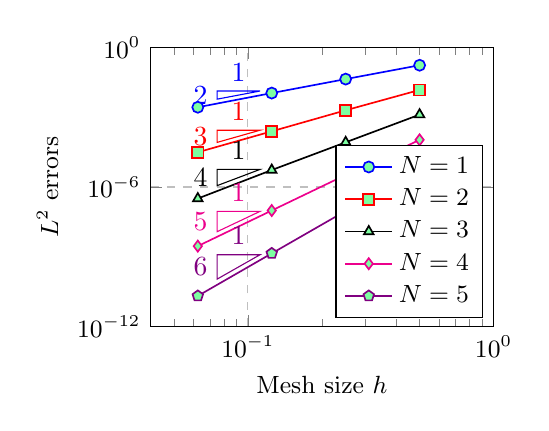
\begin{tikzpicture}
\begin{loglogaxis}[
	legend cell align=left,
	width=.49\textwidth,
    xlabel={Mesh size $h$},
       ylabel={$L^2$ errors}, 
    xmin=.04, xmax=1,
    ymin=1e-12, ymax=1,
    legend pos=south east,
    xmajorgrids=true,
    ymajorgrids=true,
    grid style=dashed,
] 

\addplot[color=blue,mark=*,semithick, mark options={fill=markercolor}]
coordinates{(0.5,0.1732)(0.25,0.0439)(0.125,0.0110)(0.0625,0.0027)};
%\node at (axis cs:.04,.0027) {$N = 1$};

\logLogSlopeTriangleFlip{0.32}{0.125}{0.815}{2}{blue}

\addplot[color=red,mark=square*,semithick, mark options={fill=markercolor}]
coordinates{(0.5,0.0150)(0.25,0.0020)(0.125,2.4911e-04)(0.0625,3.1277e-05)};
%\node at (axis cs:.04,3e-5) {$N = 2$};

\logLogSlopeTriangleFlip{0.32}{0.125}{0.66}{3}{red}

\addplot[color=black,mark=triangle*,semithick, mark options={fill=markercolor}]
coordinates{(0.5, 0.0013)(0.25,8.3910e-05)(0.125,5.3840e-06)(0.0625,3.2015e-07)};
%\node at (axis cs:.04,3e-7) {$N = 3$};

\logLogSlopeTriangleFlip{0.32}{0.125}{0.505}{4}{black}

\addplot[color=magenta,mark=diamond*,semithick, mark options={fill=markercolor}]
coordinates{(0.5,1.0687e-04)(0.25,3.3041e-06)(0.125,9.7715e-08)(0.0625, 2.8750e-09)};
%\node at (axis cs:.03,1.5e-13) {$a = 10^{-4}$};
\logLogSlopeTriangleFlip{0.32}{0.125}{0.34}{5}{magenta}

\addplot[color=violet,mark=pentagon*,semithick, mark options={fill=markercolor}]
coordinates{(0.5,5.9754e-06)(0.25,9.3644e-08)(0.125,1.3980e-09)(0.0625,2.0686e-11)};

\logLogSlopeTriangleFlip{0.32}{0.125}{0.17}{6}{violet}

%\node at (axis cs:.03,6.8e-10) {$u$ discontinuous};
\legend{$N=1$,$N=2$,$N=3$,$N=4$,$N=5$}
\end{loglogaxis}
\end{tikzpicture}
\caption{Convergence of $L^2$ errors for harmonic oscillation.}
\label{fig:harmonic_osc}
\end{figure}

\subsubsection{Rayleigh and Lamb waves}  

Next, we examine the convergence of WADG for Rayleigh and Lamb waves, both of which test the imposition of traction-free boundary conditions.  

Rayleigh waves are elastic surface waves which decay exponentially away from the surface.  These waves are given by the displacement vector
\begin{align*}
\bm{v}\LRp{x,y,t} &= e^{-\omega x \sqrt{1-\xi^2}}
\LRp{
\begin{array}{c}
\cos(\omega(y+c_r t)) \\
\sqrt{1-\xi^2}\sin(\omega(y+c_r t))
\end{array}
}\\
&+ \LRp{\frac{\xi^2}{2}-1}e^{-\omega x\sqrt{1-\frac{\xi^2\mu}{2\mu + \lambda}}}
\LRp{
\begin{array}{c}
\cos(\omega(y + c_r t))\\
{\sin(\omega(y+c_r t))}/{\sqrt{1-\frac{\xi^2\mu}{2\mu + \lambda}}}
\end{array}
},
\end{align*}
where $\omega$ is the wavespeed, $c_r$ is the Rayleigh phase velocity $c_r = \xi \sqrt{\mu}$, and $\xi$ satisfies
\[
\sqrt{1-\xi^2}\sqrt{1 - \frac{\xi^2\mu}{2\mu+\lambda}} - \LRp{\frac{\xi^2}{2}-1}^2 = 0.
\]
In our computations, we use $\rho = \mu = \lambda = 1$, $\xi = 0.949554083888034$, and $\omega = 2\pi$.  We solve on the domain $[0,2]\times[0,1]$ using a sequence of uniform triangular meshes, and enforce traction-free boundary conditions at $x=0$ and exact Dirichlet boundary conditions at $x=2$.  Periodic boundary conditions are applied at $y = 0$ and $y = 1$.  

Lamb waves are supported by elastic waveguides with traction-free (free surface) boundary conditions at the top and bottom of the domain.  The displacement of these waves 
\begin{align*}
\bm{v}_1\LRp{x,y,t} &= \LRp{-kB_1 \cos(p y)- qB_2 \cos(q y)} \sin(k x - \omega t)\\
\bm{v}_2\LRp{x,y,t} &= \LRp{-pB_1 \sin(py) + kB_2 \sin(qy)} \cos(kx - \omega t)
\end{align*}
where $k$ is the wavenumber and $\omega$ is the frequency, and the constants $p$ and $q$ are defined as
\[
p^2 = \frac{\omega^2}{2\mu + \lambda} - k^2, \qquad q^2 = \frac{\omega^2}{\mu} - k^2.
\]
The wavenumber $k$ and frequency $\omega$ are related through a dispersion relation.  The ratio of the amplitudes $B_1/ B_2$ can be determined using other parameters, implying that $B_1, B_2$ are unique up to a scaling constant.  In our experiments, we use $\rho = \mu = 1$, $\lambda = 2$, $k = 2\pi$.  For these values, $\omega = 13.137063197233$, $B_1 = 126.1992721468$ and $B_2 = 53.88807700007$.  We solve on the domain $[-1,1]\times[-1/2,1/2]$, with traction-free boundary conditions at $y = \pm 1/2$ and periodic boundary conditions at $x = \pm 1$.  

Figure~\ref{fig:rayleigh} shows $L^2$ errors for both waves at time $T = 1$.  Observed convergence rates fall between the optimal rate of $O(h^{N+1})$ and theoretical rate of $O(h^{N+1/2})$ \cite{johnson1986analysis}.  

\begin{figure}
\centering
\subfloat[Rayleigh wave]{
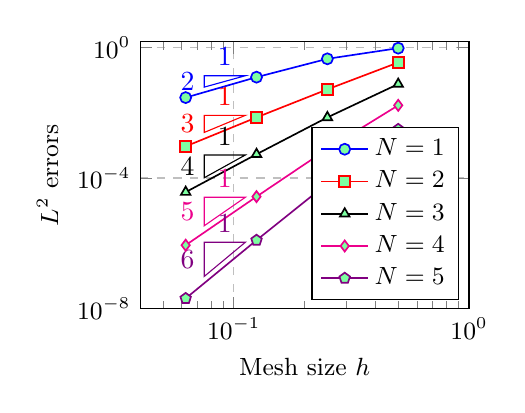
\begin{tikzpicture}
\begin{loglogaxis}[
    legend cell align=left,
    width=.475\textwidth,
    xlabel={Mesh size $h$},
    ylabel={$L^2$ errors}, 
    xmin=.04, xmax=1,
    ymin=1e-8, ymax=1.5,
    legend pos=south east,
    xmajorgrids=true,
    ymajorgrids=true,
    grid style=dashed,
] 

\addplot[color=blue,mark=*,semithick, mark options={fill=markercolor}]
coordinates{(0.5,0.9569)(0.25,0.4509)(0.125,0.1234)(0.0625,0.0292)};%\node at (axis cs:.04,.0027) {$N = 1$};
\logLogSlopeTriangleFlip{0.32}{0.125}{0.83}{2}{blue}

\addplot[color=red,mark=square*,semithick, mark options={fill=markercolor}]
coordinates{(0.5,0.3483)(0.25,0.0521)(0.125,0.0072)(0.0625,9.3104e-04)};
\logLogSlopeTriangleFlip{0.32}{0.125}{0.66}{3}{red}

\addplot[color=black,mark=triangle*,semithick, mark options={fill=markercolor}]
coordinates{(0.5,0.0759)(0.25,  0.0072)(0.125,5.3457e-04)(0.0625,3.6842e-05)};
\logLogSlopeTriangleFlip{0.32}{0.125}{0.49}{4}{black}

\addplot[color=magenta,mark=diamond*,semithick, mark options={fill=markercolor}]
coordinates{(0.5,0.0169)(0.25,  7.7478e-04)(0.125,2.6817e-05)(0.0625,8.6998e-07)};
\logLogSlopeTriangleFlip{0.32}{0.125}{0.31}{5}{magenta}

\addplot[color=violet,mark=pentagon*,semithick, mark options={fill=markercolor}]
coordinates{(0.5,0.0031)(0.25,6.7730e-05)(0.125,1.235333472480438e-06)(0.0625,2.023726469227763e-08)};

\logLogSlopeTriangleFlip{0.32}{0.125}{0.12}{6}{violet}

%\node at (axis cs:.03,6.8e-10) {$u$ discontinuous};
\legend{$N=1$,$N=2$,$N=3$,$N=4$,$N=5$}
\end{loglogaxis}
\end{tikzpicture}
}
\subfloat[Lamb wave]{
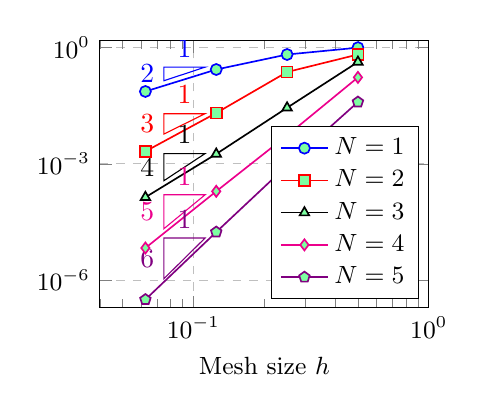
\begin{tikzpicture}
\begin{loglogaxis}[
	legend cell align=left,
	width=.475\textwidth,
    xlabel={Mesh size $h$},
%       ylabel={$L^2$ errors}, 
    xmin=.04, xmax=1,
    ymin=2e-7, ymax=1.5,
    legend pos=south east,
    xmajorgrids=true,
    ymajorgrids=true,
    grid style=dashed,
] 

\addplot[color=blue,mark=*,semithick, mark options={fill=markercolor}]
coordinates{(0.5,0.9924)(0.25,0.6613)(0.125,0.2713)(0.0625,0.0737)};%\node at (axis cs:.04,.0027) {$N = 1$};
\logLogSlopeTriangleFlip{0.32}{0.125}{0.85}{2}{blue}

\addplot[color=red,mark=square*,semithick, mark options={fill=markercolor}]
coordinates{(0.5,0.6614)(0.25,0.2338)(0.125,0.0205)(0.0625,0.0021)};
\logLogSlopeTriangleFlip{0.32}{0.125}{0.65}{3}{red}

\addplot[color=black,mark=triangle*,semithick, mark options={fill=markercolor}]
coordinates{(0.5,0.4237)(0.25, 0.0280)(0.125, 0.0018)(0.0625,1.3754e-04)};
\logLogSlopeTriangleFlip{0.32}{0.125}{0.475}{4}{black}

\addplot[color=magenta,mark=diamond*,semithick, mark options={fill=markercolor}]
coordinates{(0.5, 0.1700 )(0.25,0.0054 )(0.125,1.9613e-04)(0.0625,6.7755e-06)};
\logLogSlopeTriangleFlip{0.32}{0.125}{0.295}{5}{magenta}

\addplot[color=violet,mark=pentagon*,semithick, mark options={fill=markercolor}]
coordinates{(0.5, 0.0393)(0.25,9.0649e-04)(0.125, 1.7466e-05)(0.0625,3.1730e-07)};
\logLogSlopeTriangleFlip{0.32}{0.125}{0.1075}{6}{violet}

%\node at (axis cs:.03,6.8e-10) {$u$ discontinuous};
\legend{$N=1$,$N=2$,$N=3$,$N=4$,$N=5$}
\end{loglogaxis}
\end{tikzpicture}
\label{fig:rayleigh}
}
\caption{Convergence of $L^2$ errors for Rayleigh and Lamb wave solutions.}
\end{figure}

\subsubsection{Rayleigh waves in near-incompressible materials}
\label{sec:incomp}

As noted in Section~\ref{sec:wadgelas}, error estimates for isotropic elasticity no longer hold in the incompressible limit with $\mu / \lambda \rightarrow 0$ limit due to the fact that $\bm{C}$ becomes singular.  We use the propagation of Rayleigh waves to examine the behavior of WADG for near-incompressible materials.  We follow \cite{sjogreen2012fourth,appelo2015energy} and fix $\lambda = 1$ and set $\mu = 1, .1, .01, .001, .0001$.  Since the Rayleigh wave propagates with speed proportional to $\sqrt{\mu}$, we compute $L^2$ errors at the final time $1 / (4\sqrt{\mu})$ to ensure a fair comparison between solutions at different values of $\mu$.  

%Table~\ref{tab:incomp} shows total relative errors and relative errors for $\bm{v}$, $\bm{\sigma}$ individually at different orders and mesh sizes.  While the relative errors for $\bm{\sigma}$ grow as $\mu/\lambda \rightarrow 0$, total errors and errors for $\bm{v}$ remain roughly the same magnitude for all values of $\mu$.  
Table~\ref{tab:incomp} shows relative errors for $\bm{v}$, $\bm{\sigma}$ at different orders and mesh sizes.  The relative errors for $\bm{\sigma}$ grow as $\mu/\lambda \rightarrow 0$.  This is not surprising, as the constant in the error estimates of Section~\ref{sec:mwadgprop} blows up in the incompressible limit.  However, because the magnitude of $\bm{\sigma}$ also decreases as $\mu/\lambda\rightarrow 0$, relative errors for $\bm{v}$ remain roughly the same magnitude as the material approaches incompressibility.

\begin{table}
\centering
\subfloat[Relative error in $\bm{v}$]{
\begin{tabular}{|c||c|c|c|c|c|}
\hline
 & $\mu = 1$ & $\mu = .1$ & $\mu = .01$ & $\mu = .001$ & \mu = .0001$  \\
\hhline{|=|=|=|=|=|=|}
$N = 2$, $h = 1/4$ &  0.0288 &  0.0270 &  0.0309 & 0.0401 & 0.0568\\
\hline
$N = 3$, $h = 1/4$ & 0.0030 & 0.0027 &0.0030 & 0.0037 & 0.0049\\
\hline
$N = 4$, $h = 1/4$ & 2.7705e-04 & 2.5060e-04 & 2.9185e-04 &3.9779e-04 &5.2470e-04\\
\hhline{|=|=|=|=|=|=|}
$N = 2$, $h = 1/8$ & 0.0028  & 0.0025  & 0.0029 & 0.0036 & 0.0047 \\
\hline
$N = 3$, $h = 1/8$ & 1.8315e-04 & 1.6960e-04 &1.8524e-04 &2.2522e-04 & 2.8301e-04\\
\hline
$N = 4$, $h = 1/8$ & 8.2285e-06 & 7.5813e-06 &8.1174e-06 & 1.0762e-05&1.4886e-05\\
\hline
\end{tabular}
}\\
\subfloat[Relative error in $\bm{\sigma}$]{
\begin{tabular}{|c||c|c|c|c|c|}
\hline
 & $\mu = 1$ & $\mu = .1$ & $\mu = .01$ & $\mu = .001$& \mu = .0001$ \\
\hhline{|=|=|=|=|=|=|}
$N = 2$, $h = 1/4$ & 0.0656 &  0.0754 &  0.1214 & 0.2134 & 0.4145\\
\hline
$N = 3$, $h = 1/4$ & 0.0091 & 0.0108 & 0.0182 & 0.0321& 0.0576\\
\hline
$N = 4$, $h = 1/4$ & 9.7408e-04 & 0.0012 &  0.0022 & 0.0041 &0.0068\\
\hhline{|=|=|=|=|=|=|}
$N = 2$, $h = 1/8$ & 0.0093 & 0.0116 &0.0204  & 0.0379 &0.0765  \\
\hline
$N = 3$, $h = 1/8$ & 6.8288e-04 & 8.0145e-04 & 0.0015 & 0.0031 &0.0056\\
\hline
$N = 4$, $h = 1/8$ &3.4231e-05 &  4.3510e-05 & 8.8747e-05 & 1.9771e-04& 3.6053e-04 \\
\hline
\end{tabular}
}
%\\
%\subfloat[Total relative error ]{
%\begin{tabular}{|c||c|c|c|c|c|}
%\hline
% & $\mu = 1$ & $\mu = .1$ & $\mu = .01$ & $\mu = .001$ & \mu = .0001$ \\
%\hhline{|=|=|=|=|=|=|}
%$N = 2$, $h = 1/4$ & 0.0539 & 0.0369  &  0.0339 & 0.0409 & 0.0571\\
%\hline
%$N = 3$, $h = 1/4$ & 0.0073 & 0.0046 &0.0037 &0.0039 & 0.0050\\
%\hline
%$N = 4$, $h = 1/4$ & 7.7419e-04 & 4.8735e-04 & 3.9193e-04 &4.2768e-04 &5.3111e-04\\
%\hhline{|=|=|=|=|=|=|}
%$N = 2$, $h = 1/8$ & 0.0074 & 0.0048  & 0.0038 &  0.0038 & 0.0048  \\
%\hline
%$N = 3$, $h = 1/8$ & 5.4120e-04 & 3.2760e-04 &2.6070e-04 & 2.5465e-04 & 2.9104e-04\\
%\hline
%$N = 4$, $h = 1/8$ & 2.7006e-05 & 1.7103e-05 &1.3344e-05 &1.3133e-05&1.5507e-05\\
%\hline
%\end{tabular}
%}
\caption{Behavior of WADG for linear elastic wave propagation in the incompressible limit as $\mu / \lambda \rightarrow 0$.  Errors are shown for various orders and mesh resolutions.  }
\label{tab:incomp}
\end{table}

%\note{Examine energy stability as $\mu/\lambda\rightarrow 0$.  Matrix $\bm{C}$ becomes singular.}

\subsubsection{Stoneley waves} 

A Stoneley wave is supported along the interface between two solids \cite{stoneley1924elastic}.  Like Rayleigh waves, Stoneley waves decay exponentially away from the interface, and test the effectiveness of numerical fluxes across interfaces.  We follow \cite{wilcox2010high,appelo2015energy} and use discontinuous media defined by
\[
(\rho,\lambda,\mu) = \begin{cases}
(10 ,3,3) & y > 0\\
(1,1,1) & y < 0.
\end{cases}.
\]
The displacement vector for a Stoneley wave is then given by
\begin{align*}
\bm{v}_1(x,y,t) &= \begin{cases}
{\rm Re}\LRp{\LRp{ikB_1e^{-kb_{1p}y} + kb_{1s}B_2 e^{-kb_{1s}y}}e^{i(ky-\omega t)}}, & y > 0\\
{\rm Re}\LRp{\LRp{-k b_{1p}B_1e^{-k b_{1p} y} + i kB_2e^{-kb_{1s}y}}e^{i(kx-\omega t)}}, & y < 0
\end{cases}\\
\bm{v}_2(x,y,t) &= \begin{cases}
{\rm Re}\LRp{\LRp{ikB_3 e^{k b_{2p} y} - kb_{2s}B_4 e^{k b_{2s}y }} e^{i(kx-\omega t)}}, & y > 0\\
{\rm Re}\LRp{\LRp{k b_{2p} B_3 e^{k b_{2p}y} + ikB_4 e^{k b_{2s}y}}e^{i(kx-\omega t)}}, & y < 0
\end{cases},
\end{align*}
where $c_{st}$ is the Stoneley wave speed, and 
\[
k = \omega/ c_{st}, \qquad b_{jp} = \sqrt{1 - \frac{c_{st}^2}{(2\mu_j + \lambda_j)/\rho_j}}, \qquad  b_{js} = \sqrt{1 - \frac{c_{st}^2}{(\mu_j)/\rho_j}}, \qquad j = 1,2.
\]
The Stoneley wave speed $c_{st}$ can be determined based material parameters and interface conditions, and the amplitudes $B_1,B_2,B_3,B_4$ are determined from $c_{st}$ up to scaling by a constant.  For the parameters used in this study, we take $c_{st} = 0.546981324213884$, $B_1 = i0.2952173626624, B_2 = -0.6798795208473, B_3 = i0.5220044931212$, and $B_4 = -0.9339639688697$.  We assume $k =1$, which gives $\omega=c_{st}$.  

We solve on the domain $[-1,1]\times [-5,5]$, and enforce Dirichlet boundary conditions at all boundaries using the exact solution.  Figure~\ref{fig:stoneley} shows $L^2$ errors for two uniform meshes of triangles constructed by bisecting a quadrilateral mesh of $K_{\rm 1D} \times 5K_{\rm 1D}$ elements. Figure~\ref{subfig:stoneley1} shows errors when $K_{\rm 1D}$ is even and the mesh is fitted to the interface at $y = 0$, while Figure~\ref{subfig:stoneley2} shows errors when $K_{\rm 1D}$ is odd and the interface cuts through element interiors.  When the mesh is fitted to the interface, we observe optimal $O(h^{N+1})$ rates of convergence for $N > 1$.  

When the mesh is not fitted to the interface exactly, we compute the application of the weight-adjusted mass matrix inverse using a quadrature rule from Xiao and Gimbutas \cite{xiao2010quadrature} which is exact for degree $2N+1$ polynomials.  Since the values of $\rho,\mu$, and $\lambda$ are positive at all quadrature points, the method is energy stable.  However, since the exact solution is discontinuous, we expect an $O(1)$ error in elements cut by the interface, resulting in $L^2$ errors which converge at rate $O(h^{1/2})$.  We note that, when using piecewise constant approximations of $\mu$ and $\lambda$, we observe the same $O(h^{1/2})$ convergence rate, though errors are roughly twice as large in magnitude.  \note{Discuss possibly extending theory for WADG to low regularity weights.}  

\begin{figure}
\centering
\subfloat[Fitted interface]{
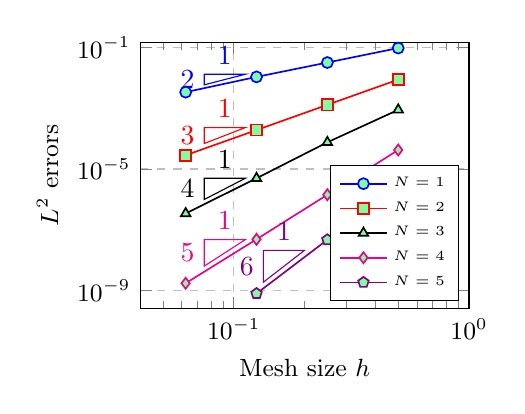
\begin{tikzpicture}
\begin{loglogaxis}[
    legend cell align=left,
    legend style={legend pos=south east, font=\tiny},
    width=.475\textwidth,
    xlabel={Mesh size $h$},
    ylabel={$L^2$ errors}, 
    xmin=.04, xmax=1,
    ymin=2.5e-10, ymax=.15,
    xmajorgrids=true,
    ymajorgrids=true,
    grid style=dashed,
] 

\addplot[color=blue,mark=*,semithick, mark options={fill=markercolor}]
coordinates{(0.5,0.0961)(0.25,0.0321)(0.125,0.0108)(0.0625,0.0034)}; 
\logLogSlopeTriangleFlip{0.32}{0.125}{0.84}{2}{blue}

\addplot[color=red,mark=square*,semithick, mark options={fill=markercolor}]
coordinates{(0.5,0.0088)(0.25,0.0013)(0.125,1.9177e-04)(0.0625, 2.8444e-05)};
\logLogSlopeTriangleFlip{0.32}{0.125}{0.62}{3}{red}

\addplot[color=black,mark=triangle*,semithick, mark options={fill=markercolor}]
coordinates{(0.5, 8.9050e-04)(0.25,7.5838e-05)(0.125,4.9595e-06)(0.0625,3.4440e-07)};
\logLogSlopeTriangleFlip{0.32}{0.125}{0.41}{4}{black}

\addplot[color=magenta,mark=diamond*,semithick, mark options={fill=markercolor}]
coordinates{(0.5,4.2348e-05)(0.25, 1.4232e-06)(0.125, 4.8606e-08)(0.0625,1.7358e-09)};
\logLogSlopeTriangleFlip{0.32}{0.125}{0.16}{5}{magenta}

\addplot[color=violet,mark=pentagon*,semithick, mark options={fill=markercolor}]
coordinates{(0.5,2.7994e-06)(0.25,4.6958e-08)(0.125,7.9344e-10)};
\logLogSlopeTriangleFlip{0.5}{0.125}{0.1}{6}{violet}

%\node at (axis cs:.03,6.8e-10) {$u$ discontinuous};
\legend{$N=1$,$N=2$,$N=3$,$N=4$,$N=5$}
\end{loglogaxis}
\end{tikzpicture}
\label{subfig:stoneley1}
}
\subfloat[Non-fitted interface]{
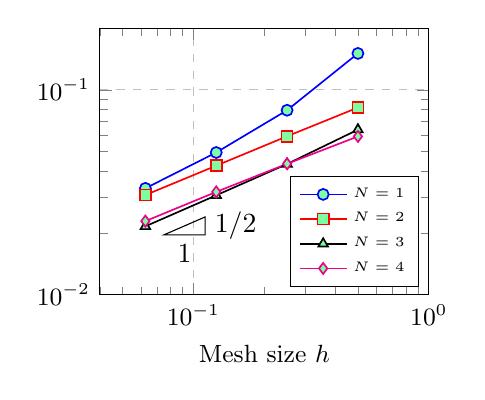
\begin{tikzpicture}
\begin{loglogaxis}[
    legend cell align=left,
    legend style={legend pos=south east, font=\tiny},
    width=.475\textwidth,
    xlabel={Mesh size $h$},
%    ylabel={$L^2$ errors}, 
    xmin=.04, xmax=1,
    ymin=1e-2, ymax=.2,
    xmajorgrids=true,
    ymajorgrids=true,
    grid style=dashed,
] 

\addplot[color=blue,mark=*,semithick, mark options={fill=markercolor}]
coordinates{(0.5,0.1507)(0.25,0.0796)(0.125,0.0495)(0.0625,0.0331)}; 
%\logLogSlopeTriangleFlip{0.32}{0.125}{0.84}{1}{blue}

\addplot[color=red,mark=square*,semithick, mark options={fill=markercolor}]
coordinates{(0.5,0.0820)(0.25,0.0594)(0.125,0.0427)(0.0625, 0.0307)};
%\logLogSlopeTriangleFlip{0.32}{0.125}{0.62}{3}{red}

\addplot[color=black,mark=triangle*,semithick, mark options={fill=markercolor}]
coordinates{(0.5, 0.0640)(0.25,0.0435)(0.125,0.0306)(0.0625,0.0216)};
%\logLogSlopeTriangleFlip{0.32}{0.125}{0.41}{4}{black}

\addplot[color=magenta,mark=diamond*,semithick, mark options={fill=markercolor}]
coordinates{(0.5, 0.0593)(0.25, 0.0436)(0.125, 0.0318)(0.0625,0.0229)};
\logLogSlopeTriangle{0.32}{0.125}{0.225}{1/2}{black}

%\addplot[dashed,color=blue,mark=*,semithick, mark options={fill=markercolor}]
%coordinates{(0.5,0.1648)(0.25,0.0927)(0.125,0.0607)(0.0625,0.0417)}; 
%
%\addplot[dashed,color=red,mark=square*,semithick, mark options={fill=markercolor}]
%coordinates{(0.5,0.1200)(0.25, 0.0855)(0.125,0.0597)(0.0625,0.0421)};
%
%\addplot[dashed,color=black,mark=triangle*,semithick, mark options={fill=markercolor}]
%coordinates{(0.5, 0.1399)(0.25,0.0942)(0.125,0.0660)(0.0625,0.0463)};
%
%\addplot[dashed,color=magenta,mark=diamond*,semithick, mark options={fill=markercolor}]
%coordinates{(0.5,0.1410)(0.25, 0.0984)(0.125, 0.0697)(0.0625, 0.0490)};



%\addplot[color=violet,mark=pentagon*,semithick, mark options={fill=markercolor}]
%coordinates{(0.5,2.7994e-06)(0.25,4.6958e-08)(0.125,7.9344e-10)};
%\logLogSlopeTriangleFlip{0.5}{0.125}{0.1}{6}{violet}

%\node at (axis cs:.03,6.8e-10) {$u$ discontinuous};
\legend{$N=1$,$N=2$,$N=3$,$N=4$}
\end{loglogaxis}
\end{tikzpicture}
\label{subfig:stoneley2}
}
\caption{Convergence of WADG for a Stoneley wave using a fitted mesh aligned with the interface and a non-fitted mesh where the interface does not lie exactly on an element boundary. }
\label{fig:stoneley}
\end{figure}

\subsubsection{Harmonic oscillation of an annulus}

This example tests the convergence of WADG for curvilinear mappings.  

\subsection{Application examples}

\subsubsection{Stiff inclusion}

Leveque stiff inclusion example.  

\subsubsection{Heterogeneous anisotropic material}

From \cite{de2007arbitrary}: discontinuous media with anisotropy on one side, isotropy on the other.

Also do a similar case where random noise is added to both sides and the anisotropy is more strongly discontinuous.  

\subsection{Three-dimensional example}

Add GPU computations here.   

\section{Conclusions}

Generally applicable to problems with spatially varying matrices $\bm{A}_{0}(\bm{x})$, such as in Maxwell's equations for cloaking problems \cite{li2012time}, as well as in vector-valued $H({\rm div})$ or $H({\rm curl})$ functions under matrix-valued mappings such as Piola transforms.  

Extension to hybrid meshes in 3D, care must be taken with pyramids \cite{chan2015orthogonal,chan2015gpu}.

which can be further accelerated by exploiting structure under Bernstein-Bezier bases \cite{chan2015gpu}. 
Formulation allows for the reduction of constant-coefficient RHS costs at high orders using BBDG \cite{chan2015bbdg}.  

\section{Acknowledgments}

The author gratefully thanks Thomas Hagstrom, Tim Warburton, Axel Modave, and Ruichao Ye for helpful and informative discussions.  

\bibliographystyle{unsrt}
\bibliography{dgpenalty}


\end{document}


